\documentclass[14pt,a4paper]{report}  %紙張設定
\usepackage{xeCJK}%中文字體模組
\setCJKmainfont{標楷體} %中文字體
\usepackage{amsmath,amssymb}%數學公式、符號
\usepackage{graphicx, subfig}%圖形
\usepackage{graphicx, subfig}%圖片模組
\usepackage{type1cm} %調整字體絕對大小
\usepackage{textpos} %設定文字絕對位置
\usepackage[top=2.5truecm,bottom=2.5truecm,
left=3truecm,right=2.5truecm]{geometry}
\usepackage{titlesec} %目錄標題設定模組
\usepackage{titletoc} %目錄內容設定模組
\usepackage{caption} %圖片標題設定
\usepackage{CJK} %中文模組
\usepackage{CJKnumb} %中文數字模組
%\usepackage{wallpaper} %浮水印
\usepackage{float}
\usepackage{enumerate}
\usepackage{listings} %引用程式碼
\usepackage{indentfirst}
\usepackage{diagbox}%引用表格

\lstset{language=Python, %設定語言
		basicstyle=\footnotesize, 
		frame=lines,
		caption={Python code}, %設定capion
		label={lst:example} %設定label
		}
\renewcommand{\baselinestretch}{1.0} %設定行距1.0

\newcommand{\thirty}{\fontsize{30pt}\baselineskip\selectfont}%字體大小30pt
\newcommand{\twentyfour}{\fontsize{24pt}{\baselineskip}\selectfont}%字體大小24pt
\newcommand{\twenty}{\fontsize{20pt}{\baselineskip}\selectfont}%字體大小20pt
\newcommand{\eigh}{\fontsize{18pt}{\baselineskip}\selectfont}%字體大小18pt
\newcommand{\sixteen}{\fontsize{16pt}{\baselineskip}\selectfont}%字體大小16pt
\newcommand{\fourteen}{\fontsize{14pt}{\baselineskip}\selectfont}%字體大小14pt
\newcommand{\twelve}{\fontsize{12pt}{\baselineskip}\selectfont}%字體大小12pt

%設定章節標題內容
\titleformat{\chapter}[hang]{\center \twenty \bf}{\twenty 第\CJKnumber{\thechapter}章}{1em}{}[]
\titleformat{\section}[hang]{\raggedright \eigh \bf}{\eigh 第{\thesection}節}{1em}{}[]
\titleformat{\subsection}[hang]{\raggedright \sixteen \bf}{\sixteen {\thesubsection}}{1em}{}[]
%章節間距
\titlespacing*{\chapter} {0pt}{0pt}{18pt}
\titlespacing*{\section} {0pt}{12pt}{6pt}
\titlespacing*{\subsection} {0pt}{6pt}{6pt}
%設定目錄內容
\titlecontents{chapter}[11mm]{}{\normalfont\fontsize{14pt}{2.5pt}\bfseries\makebox[3.5em][l]
{第\CJKnumber{\thecontentslabel}章}}{}{\titlerule*[0.7pc]{.}\contentspage}
\titlecontents{section}[18mm]{}{\fourteen \makebox[2em][l]
{\fourteen \thecontentslabel}}{}{\titlerule*[0.7pc]{.}\contentspage}
\titlecontents{subsection}[25mm]{}{\fourteen \makebox[2.5em][l]{{\fourteen \thecontentslabel}}}{}{\titlerule*[0.7pc]{.}\contentspage}
%設定圖表目錄內容
\newcommand{\loflabel}{圖}
\newcommand{\lotlabel}{表}
\captionsetup{font={Large}} %設定標題大小
\captionsetup[figure]{name=圖} %固定標題名稱
\captionsetup[table]{name=表}

\begin{document}
    {\renewcommand\baselinestretch{1.4}\selectfont %設定以下行距
    {\begin{center} %以下文字置中
        \twentyfour{國立虎尾科技大學}\\{機械設計工程系}\\{專題製作報告}\\
        \hspace*{\fill} \\
        \bf \thirty {Pyslvs-UI 平面多連桿機構套件之合成與應用}\\
        {\renewcommand\baselinestretch{1.3}\selectfont %設定以下行距
        \bf \thirty {Synthesis and Application of Pyslvs-UI Planar Multi-link Mechanism Package}\\}
    \end{center}}
    \par} %結束指定行距

     {\renewcommand\baselinestretch{1.2}\selectfont %設定以下行距
    {\begin{textblock}{30}(1.45,1.1) %{寬度}(以左上角為原點之右移量,下移量)
    \noindent \eigh \makebox[6em][s]{指導教授}\enspace:\qquad
    \eigh \makebox[8em][s]{李武鉦}\\ %\noindent指定首行不進行縮排
    \eigh \makebox[6em][s]{班級}\enspace:\qquad
    \eigh \makebox[8em][s]{四設計三甲} \\ %\makebox為文本盒子
    \eigh \makebox[6em][s]{學生}\enspace:\qquad
    {\begin{minipage}[t][9.8em][s]{12em}
    \eigh \setlength{\baselineskip}{10pt plus 2pt}
    林昱秀\qquad40723102\vfill 林晏瑩\qquad40723103\vfill 劉光智\qquad40723145\vfill 吳佳穎\qquad40723153\vfill 蔡育灃\qquad40723245
    \end{minipage}}
    \end{textblock}} %指定以下文字整體偏移至頁面的絕對位置
    \par} %結束指定行距

    {\begin{textblock}{12}(0,6.8)
    {\begin{center}
    \noindent \eigh \makebox[12em][s]{中華民國一一零年四月}
    \end{center}}
    \end{textblock}}
    \newpage
%專題製作合可證明
 {\renewcommand\baselinestretch{1.4}\selectfont %設定以下行距
 {\begin{center}
    {\eigh {國立虎尾科技大學 \qquad 機械設計工程系}\\{學生專題製作合格認可證明}\\
    \hspace*{\fill} \\ %似enter鍵換行
    \par}
     \end{center}}
    {\begin{textblock}{60}(1.85,0.8)
    \noindent \fourteen 專題製作修習學生\enspace:\quad
    {\begin{minipage}[t]{10em}\underline{四設三甲\enspace 40723102\enspace 林昱秀}\\ \underline{四設三甲\enspace 40723103\enspace 林晏瑩}\\ \underline{四設三甲\enspace 40723145\enspace 劉光智}\\ \underline{四設三甲\enspace 40723153\enspace 吳佳穎}\\ \underline{四設三乙\enspace 40723245\enspace 蔡育灃}\\ %下劃線符號指令
    \end{minipage}}
         \par} %結束指定行距
    {\renewcommand\baselinestretch{1.2}\selectfont %設定以下行距
    {\begin{textblock}{30}(1.8,4)
    \noindent \fourteen 專題製作題目\enspace :\quad Pyslvs-UI 平面多連桿機構套件之合成與應用
    \hspace*{\fill} \\
    \hspace*{\fill} \\
    \noindent \fourteen 經評量合格,特此證明
    \hspace*{\fill} \\
    \hspace*{\fill} \\
    \noindent \fourteen \makebox[6em][s]{評審委員}\enspace:\quad
    {\begin{minipage}[t]{6em} \underline{            }\\ \underline{            }\\ \underline{            }\\
    \end{minipage}}
    \end{textblock}}
    {\begin{textblock}{10}(1.8,9)
    {\begin{flushleft}
    \fourteen \makebox[6em][s]{指導老師}\enspace:\quad \underline{            }\\
    \fourteen \makebox[6em][s]{系主任}\enspace:\quad \underline{            }\\
    \hspace*{\fill} \\
    \fourteen \makebox[12em][s]{中華民國一一零年}
    \fourteen \makebox[9em][s]{四月二十九日}
    \end{flushleft}}
    \end{textblock}}
    \end{textblock}}
     \par} %結束指定行距
     \newpage
%摘要
	\pagenumbering{roman} %設定以下頁碼為羅馬數字
    \addcontentsline{toc}{chapter}{\fourteen{摘要}} %將摘要加入目錄
    \begin{center}
    \twenty \bf{摘要}\\
    \end{center}
	\hspace*{\fill} \\

	\quad \fourteen {本專題利用一開源套件Pyslvs-UI進行機構尺寸合成,並以登山車避震機構作為範例,針對影響登山車騎乘舒適度及整體平衡進行防後蹲(Anti-squat)及防後升(Anti-rise)做為設計需求建立適應函數再將合成所得結果進行量化評比並探討不同避震機構類型的差異,後續將合成後的尺寸作為參數套入自行編寫的程式透過Inventor自動生成3D零件,接著將上述所建立的零件利用xml格式設定零件組合位置、零件從屬關係和動態系統的碰撞設定後匯入CoppeliaSim,最後以CoppeliaSim API控制馬達轉軸讓機構進行運動模擬。}
    
	\begin{flushleft}
	\fontsize{14pt}{2.5pt}{關鍵字:機構合成、機構分析、登山車避震機構}
	\end{flushleft}
%---目錄---%
\addcontentsline{toc}{chapter}{\fourteen{目錄}} %將目錄加入目錄
{\begin{center}
\renewcommand{\contentsname}{\centerline{\fontsize{20pt}{\baselineskip}\selectfont\textbf{目\quad 錄}}}
{\fourteen \tableofcontents}
%---圖目錄---%
\addcontentsline{toc}{chapter}{\fourteen{圖目錄}} %將圖表目錄加入目錄
\renewcommand{\listfigurename}{\centerline{\fontsize{20pt}{\baselineskip}\selectfont\textbf{圖\quad 目\quad 錄 }}}
\renewcommand{\numberline}[1]{\loflabel~#1\hspace*{1em}}
{\fourteen \listoffigures}

%---表目錄---%
\addcontentsline{toc}{chapter}{\fourteen{表目錄}} %將圖表目錄加入目錄
\renewcommand{\listtablename}{\centerline{\fontsize{20pt}{\baselineskip}\selectfont\textbf{表\quad 目\quad 錄 }}}
\renewcommand{\numberline}[1]{\lotlabel~#1\hspace*{1em}}
{\fourteen \listoftables}

\end{center}}



%---簡介---%
	{\begin{center}
	\chapter{簡介}
	\end{center}}	
\pagenumbering{arabic} %設定以下頁碼為阿拉伯數字

	\section{研究背景與動機}
      \quad \fourteen {隨著科技越來越發達網路上有許多機構分析的套件,但是鮮少有機構合成功能的套件,且大多無公開原始碼。而本專題所使用的套件-Pyslvs-UI為本研究室所開發的套件且有公開原始碼,因此本專題利用該套件驗證合成及模擬功能並以合成一登山車後避震機構為例。}
	  \\
	\section{研究目的與方法}
      \quad \fourteen {首先建立一現有登山車避震機構,再針對不影響現有自行車車架的尺寸但對於避震能力有較大影響的接頭利用遺傳演算法求解最佳位置以得到最佳連桿尺寸,接著將上述所得到的接頭位置和連桿長度利用Inventor自動產生對應連桿尺寸的零件,後續利用xml格式匯入CoppeliaSim並利用CoppeliaSim API設定馬達讓該機構進行運動模擬。上述流程如下圖所示。}
     
%---文獻探討---%
    {\begin{center}
	\chapter{文獻探討}
	\end{center}}
%-------平面機構分析套件-------%	
	\section{平面機構分析套件}
		\hspace*{\fill} \\
		\subsection{Linkage}
		\fourteen {Linkage為電腦輔助設計的應用程式,用於機械鏈接的原型製作。基本功能為設計帶有樞軸連接器或滑動連接器之機構、驅動機構的輸入可以是旋轉或線性的、可在運動的連桿上安裝齒輪和鏈條機構、將繪圖功能分配給連接點顯示其運動之軌跡。其工作介面如圖\ref{fig_Linkage:scale}所示。}
      
      	\begin{figure}[hbt!]
        \centering
        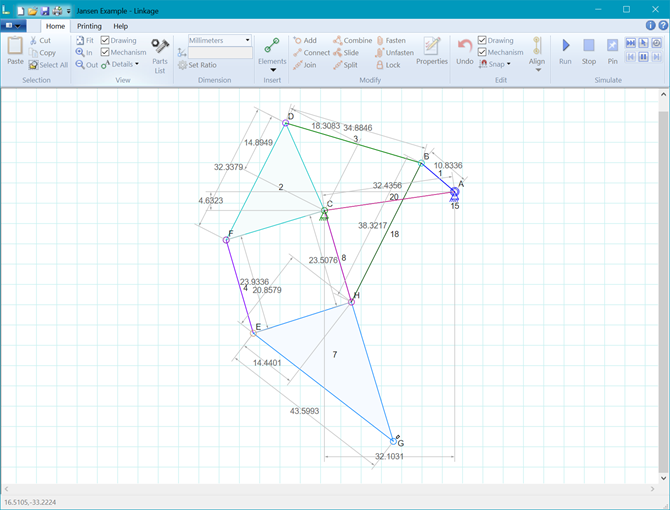
\includegraphics[scale=1]{Linkage.png}
        \caption{Linkage工作介面}
        \label{fig_Linkage:scale}
    	\end{figure}
      	\hspace*{\fill} \\   	
	  	 	
\newpage

		\subsection{M.Sketch}       
		\fourteen {M.Sketch,一種原型設計工具,設計目的在為非專業人士提供簡單直觀的界面,輕鬆學習與使用幾何圖形的模擬。工作介面如圖\ref{fig_M.Sketch:scale}所示。\\
		其中有五個主要功能:}
		
        \begin{itemize} 
        \item 繪製機構草圖:軟體介面中,藉由單擊與拖動滑鼠來簡單的繪製連桿接點,也可將接點轉換為滑塊,以此快速設計連桿機構。
        \item 運動軌跡可視化:根據馬達的旋轉值,可看到動畫上每個鏈接的坐標變化、設定欲關注之端點並給予標記,則可看到該端點預期的運動路徑。
		\item 逐步設計:首先根據繪製所需之運動機構後,使其生成機構路徑,再優化當前機構所適合的路徑。
		\item 加工支援:可導出PDF文件中每個鏈接的組合圖、示意圖和零件圖,亦可導出鏈接和關聯零件的3D模型,以匯入3D列印機等。
		\item 高可及性:M.Sketch是作為Web的應用程序開發的,用戶可以在Web瀏覽器(例如GoogleChrome)上申請帳號後,即可直接使用,無需在電腦上進行任何安裝。
		\end{itemize}  
       
 		\begin{figure}[H]
        \centering
        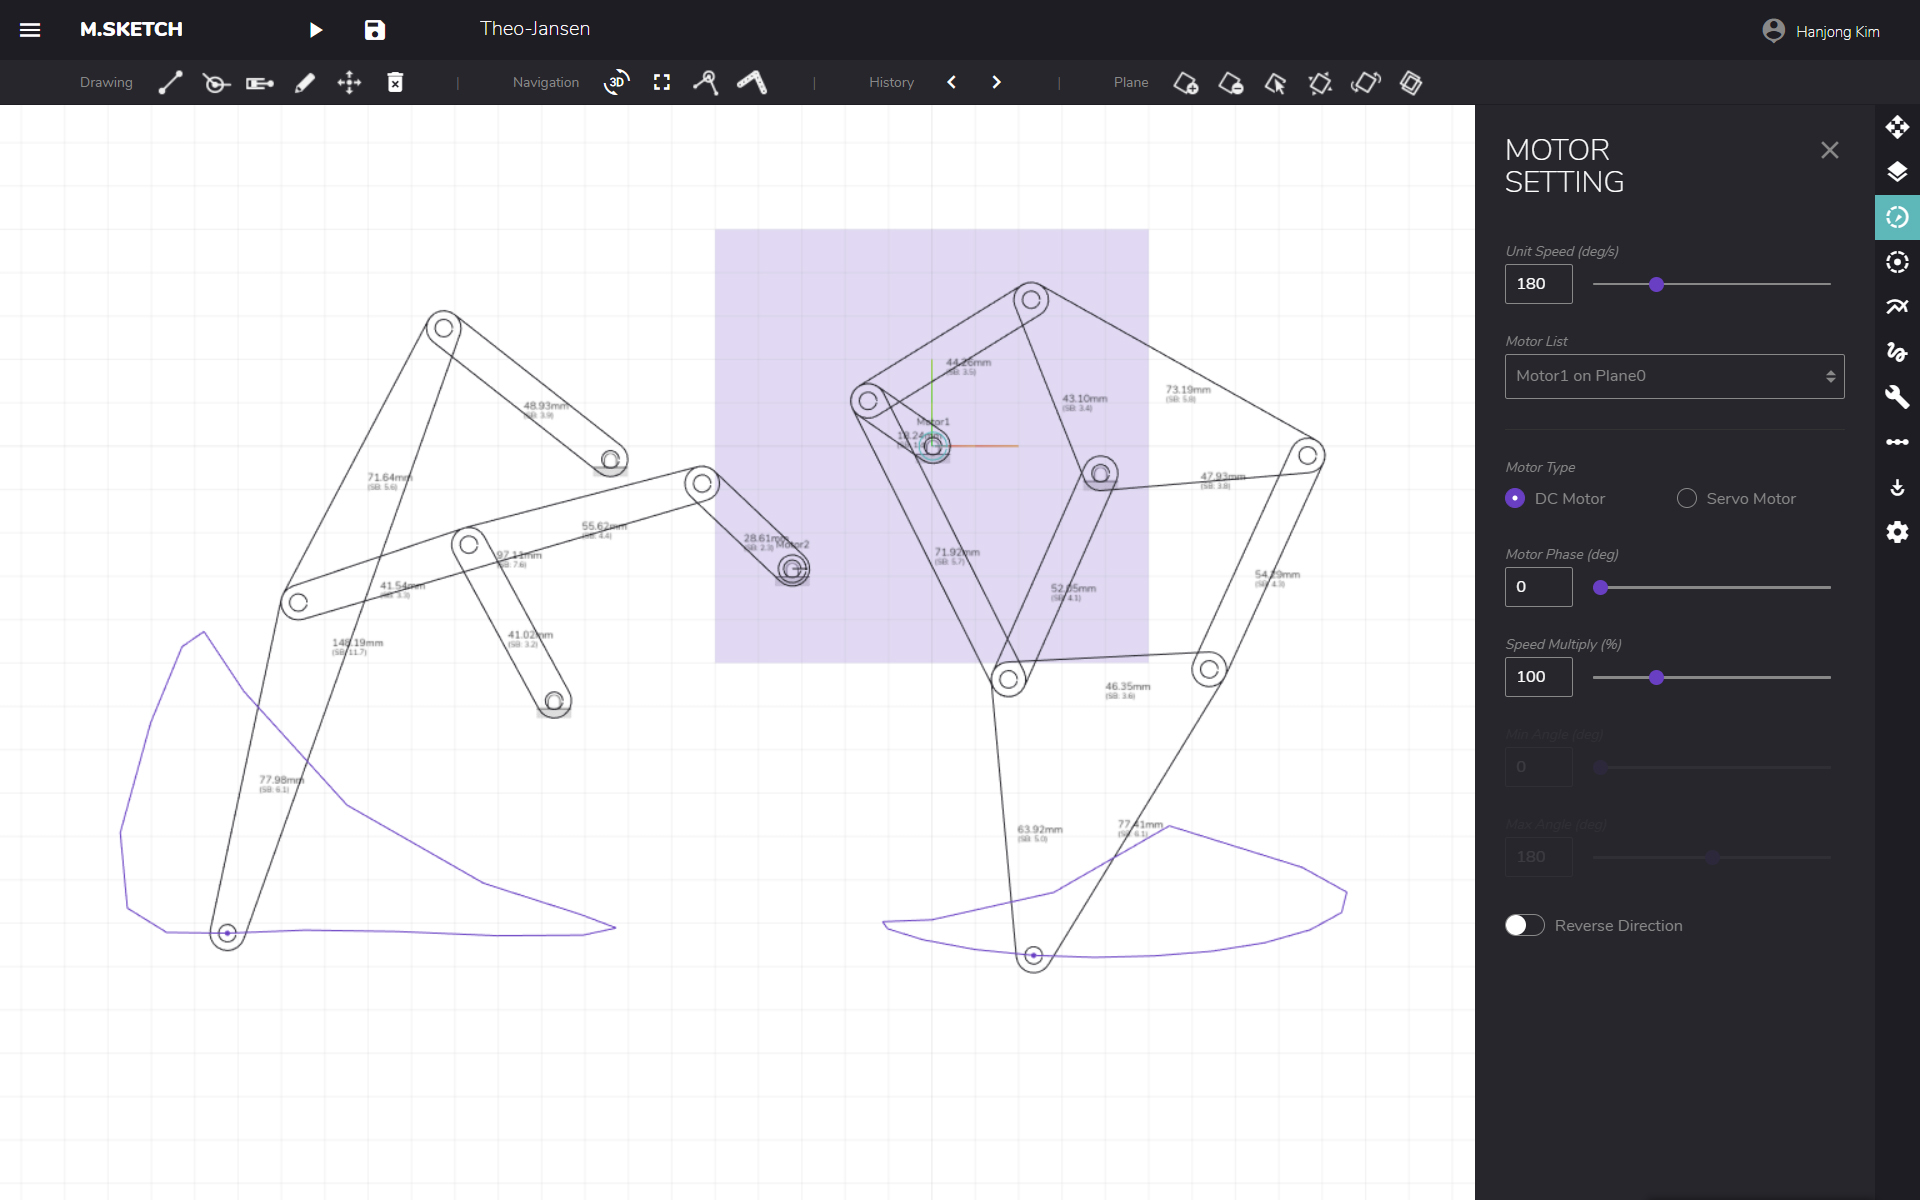
\includegraphics[scale=0.25]{M.Sketch.jpg} 
        \caption{M.Sketch工作介面} 
		\label{fig_M.Sketch:scale}
    	\end{figure}
		\hspace*{\fill} \\
\newpage

%-------平面機構合成套件-------%
	\section{平面機構合成套件}
      	\subsection{MeKin2D}
		\fourteen {MeKin2D是用Free Pascal編寫的子程序包,主要使用模組化方法對平面連桿機構進行運動學模擬,運動學模擬圖如\ref{fig_平面連桿之運動學模擬:scale}所示。\\該套件亦可以用於凸輪機構的合成和分析,以及漸開線齒輪的產生,凸輪分析圖如\ref{fig_盤式凸輪機構之合成與分析:scale}所示。\\MeKin2D的獨特功能包括:}
        \begin{itemize}
        \item 具有生成重複機構的能力。
        \item 將速度和加速度(法向和切向)顯示為向量。
        \item 將多邊形形狀附加到運動的接點。
        \item 顯示動態時線性和角度的大小。
        \item 顯示螺桿實際運作時的運動軌跡。
        \item 可以合成與分析凸輪機構。
		\end{itemize}  
		      
       	\begin{figure}[H]
		\centering
		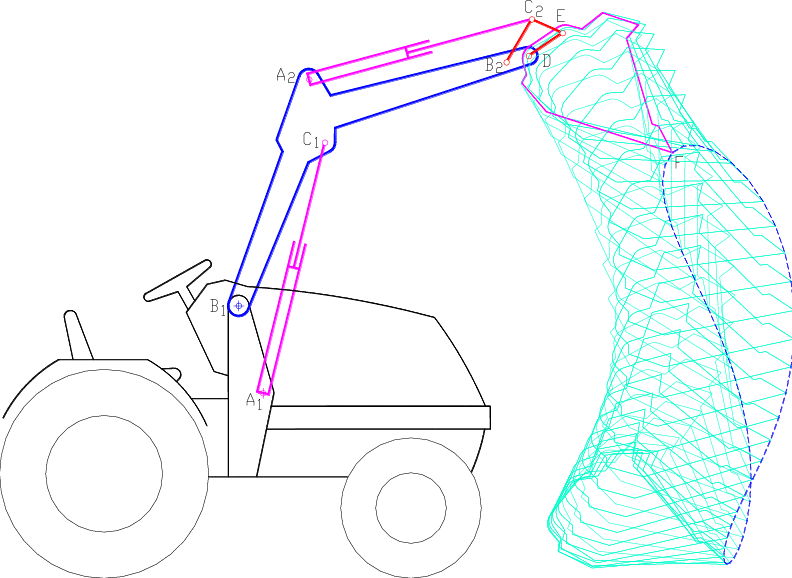
\includegraphics[scale=0.4]{平面連桿之運動學模擬.png} 
		\caption{平面連桿之運動學模擬} 
		\label{fig_平面連桿之運動學模擬:scale}
		
		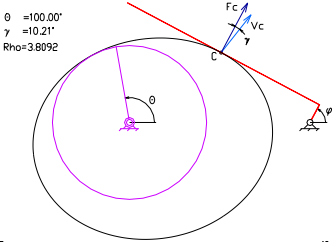
\includegraphics[scale=0.8]{盤式凸輪機構之合成與分析.png} 
		\caption{盤式凸輪機構之合成與分析} 
		\label{fig_盤式凸輪機構之合成與分析:scale}   
    	\end{figure}
		\hspace*{\fill} \\
\newpage

		\subsection{WinMecC}
		\fourteen {WinMecC為一種電腦軟件,主要用於1個自由度平面機構的分析與合成。基本功能為將機構的運動學和動力學分析之結果數值化或圖視化、可以優化分析創建的機構,依據特定點所期望遵循之路徑進行機構合成,工作介面如圖\ref{fig_WinMecC:scale}所示。}
        \begin{figure}[H]
        \centering
        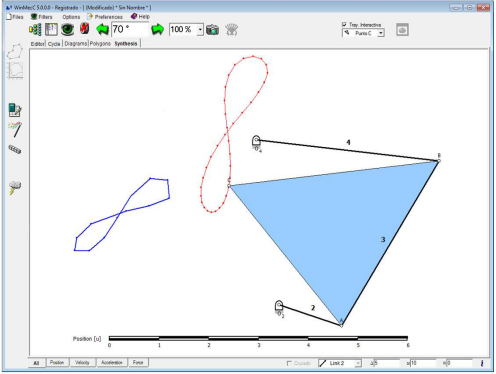
\includegraphics[scale=0.6]{WinMecC.png} 
        \caption{WinMecC} 
        \label{fig_WinMecC:scale}
    	\end{figure}
    	\hspace*{\fill} \\
    	 
		\subsection{GIM}     
		\fourteen {GIM是COMPMECH Research Group創建的註冊免費軟件,用於平面機構的運動模擬合成以及機械結構的靜態分析。GIM軟件具有三個主要模組:幾何、運動、合成。}
        \begin{itemize} 
       	\item 幾何模組:設計要分析的機構,建立其節點與元件,定義連接點的類型(旋轉接頭或滑塊),並設定固定點。
       	\item 運動模組:透過運動學分析與模擬,在運動點繪製路徑以及路徑的曲率中心,可在畫面上看到運動極點的位置、速度和加速度向量,並繪製與分析數據相關的圖形和表格。
       	\item 合成模組:依據特定點所期望之運動路徑,進行機構軌跡合成。該套件之合成介面如圖\ref{fig_GIM:scale}所示。
       	\end{itemize}
       
        \begin{figure}[H]
        \centering
        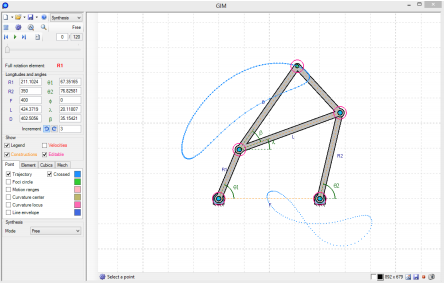
\includegraphics[scale=0.8]{GIM.png} 
        \caption{GIM合成介面} 
        \label{fig_GIM:scale}
    	\end{figure}
\newpage

%-------比較結果-------%	
	\section{比較結果}
		\fourteen {經由表\ref{tab_機構套件比較表:scale}得知,市面上雖然有很多款平面機構分析與合成套件,各個套件的功能性質也都很高級,但共同缺點是各個套件都不是開源軟體,故最終選用\underline{張元}學長所開發的\underline{Pyslvs-UI平面多連桿機構套件},運用其開源軟體的特點,來收集各套件優秀且實用的功能,進行組合與應用,來作為本專題之研究以及延伸。\\
		\hspace*{\fill} \\

		\begin{table}[htbp] %htbp代表表格浮動位置
			\centering%表格居中
			\caption{機構套件比較表}%表:標題
			\large%字體大小
			\label{tab_機構套件比較表:scale}
			\begin{tabular}{|c|c|c|c|c|c|c|}
			\hline
			\diagbox[width=9em]{功能}{套件}& Pyslvs-UI & Linkage & M.Sketch & MeKin2D & WinMecC & GIM \\ 
			\hline
			開源軟體 		&$\surd$&		&		&		&		&\\
			\hline
			編譯成可攜檔 	&$\surd$&		&		&		&		&\\
			\hline
			平面機構分析 	&$\surd$&$\surd$&$\surd$&$\surd$&$\surd$&\\
			\hline
			平面機構合成 	&$\surd$& 		&$\surd$&$\surd$&$\surd$&$\surd$\\
			\hline
			平面凸輪分析 	& 		&	    &		&$\surd$&		&\\
			\hline
			顯示運動軌跡 	&$\surd$&$\surd$&$\surd$&$\surd$&$\surd$&$\surd$\\
			\hline
			Web網頁版 	& 		&		&$\surd$&		&		&\\
			\hline
			速度/加速度向量 & 	&		&$\surd$&$\surd$&		&$\surd$\\
			\hline
			\end{tabular}
		\end{table}	
		
		
\newpage
      \section{自行車避震機構研究}
       \subsection{Single-pivot suspension(單軸懸架)}
       \hspace*{\fill} \\
       \fourteen {最簡單的懸架設計為單樞軸,使用搖臂連接後軸、主樞軸、避震器,特點在於後軸直接連接至主樞軸,避震器連接到搖臂上,搖桿環繞在主樞軸中心旋轉,槓桿比由避震器的位置決定,固定中心可在行駛過程預測懸架特性,但也意味著不同階段修改懸架特性能力有限,示意圖產品型號為 Orange Stage的 Stage 6 Factory,如圖\ref{fig_Single-pivot:scale}。}
     \begin{figure}[H]
        \centering
        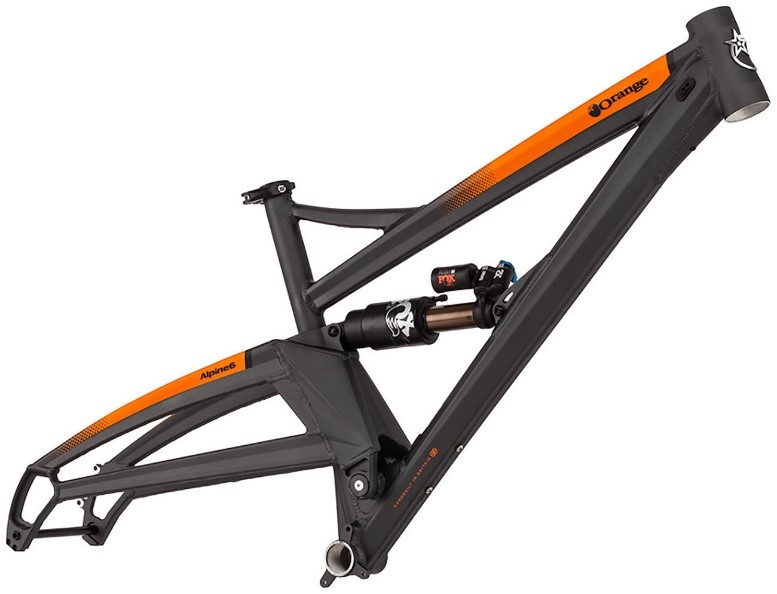
\includegraphics[scale=0.8]{單軸懸架.jpg} 
        %照片須放在和文檔相同之資料夾內
        \caption{單軸懸架} %有caption的圖才會編入目錄中
        \label{fig_Single-pivot:scale} %此處的label相當於一個圖片的專屬標誌,目的是方便上下文的引用
    \end{figure}
       \hspace*{\fill} \\
       \subsection{Linkage-driven Single-pivot suspension(連桿驅動之單樞軸懸架)}
       \hspace*{\fill} \\        
        \fourteen {如同單樞軸設計藉由後軸通過搖臂連接到主樞軸,增加聯動裝置在避震與搖臂間允許調整槓桿比率曲線,並在搖臂與避震器間建立連桿以改變槓桿比,搖臂圍繞在主軸旋轉且將中心固定於整個行程中,示意圖產品車架為Orange Stage的Orange 2020 Alpine 6 Frame 27.5,如圖\ref{fig_Linkage-driven Single-pivot:scale}。}
     \begin{figure}[H]
        \centering
        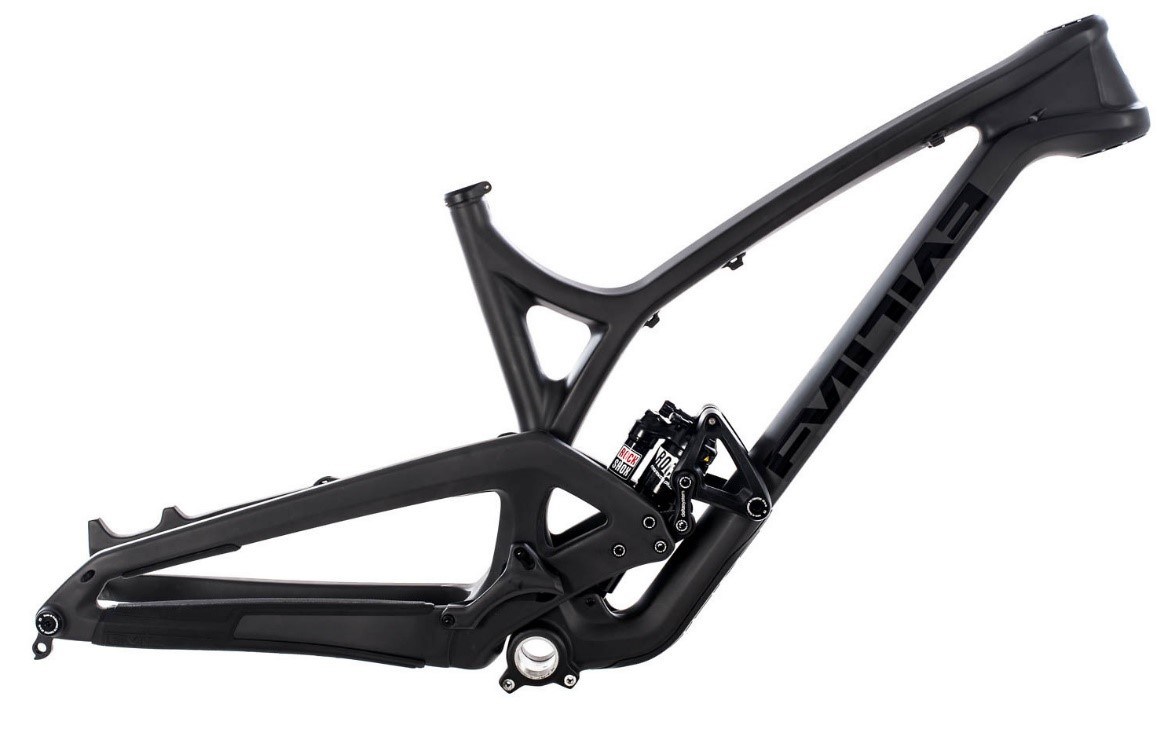
\includegraphics[scale=0.65]{連桿驅動之單樞軸懸架.jpg} 
        %照片須放在和文檔相同之資料夾內
        \caption{連桿驅動之單樞軸懸架} %有caption的圖才會編入目錄中
        \label{fig_Linkage-driven Single-pivot:scale} %此處的label相當於一個圖片的專屬標誌,目的是方便上下文的引用
    \end{figure}
        \newpage
        \subsection{High-Pivot Idler suspension(高樞轉惰輪懸架)}
        \hspace*{\fill} \\
        \fourteen{通常建構在單樞軸或鏈接驅動的單樞軸設計上,其樞軸位置位於鏈條上方,為使控制鏈條增長,鏈輪惰輪將鏈條從鏈輪佈置到主樞軸的頂部或非常靠近主樞軸的位置,主樞軸定位在鏈輪上方更高的位置,使用單樞軸同時中心在整個行程中是固定的。
         \hspace*{\fill} \\  
但是,在撞擊過程中,後搖臂在主樞軸下方以曲線向上和向後旋轉,而不是在低樞軸位置向上和向後旋轉,且後軸路徑可以幫助懸架在方形撞擊中保持平穩。
		 \hspace*{\fill} \\  
鏈條繞到惰輪上,使鏈條與樞軸和後軸成一直線,大大減少了鏈增長的影響。惰輪的位置可以由設計人員用來增加或減少防下蹲的水平,但不會改變通常較高的防起落高度,如圖\ref{fig_High-Pivot Idler:scale},產品來源為Forbidden Druid的Druid Frame – 2021。}
     \begin{figure}[hbt!]
        \centering
        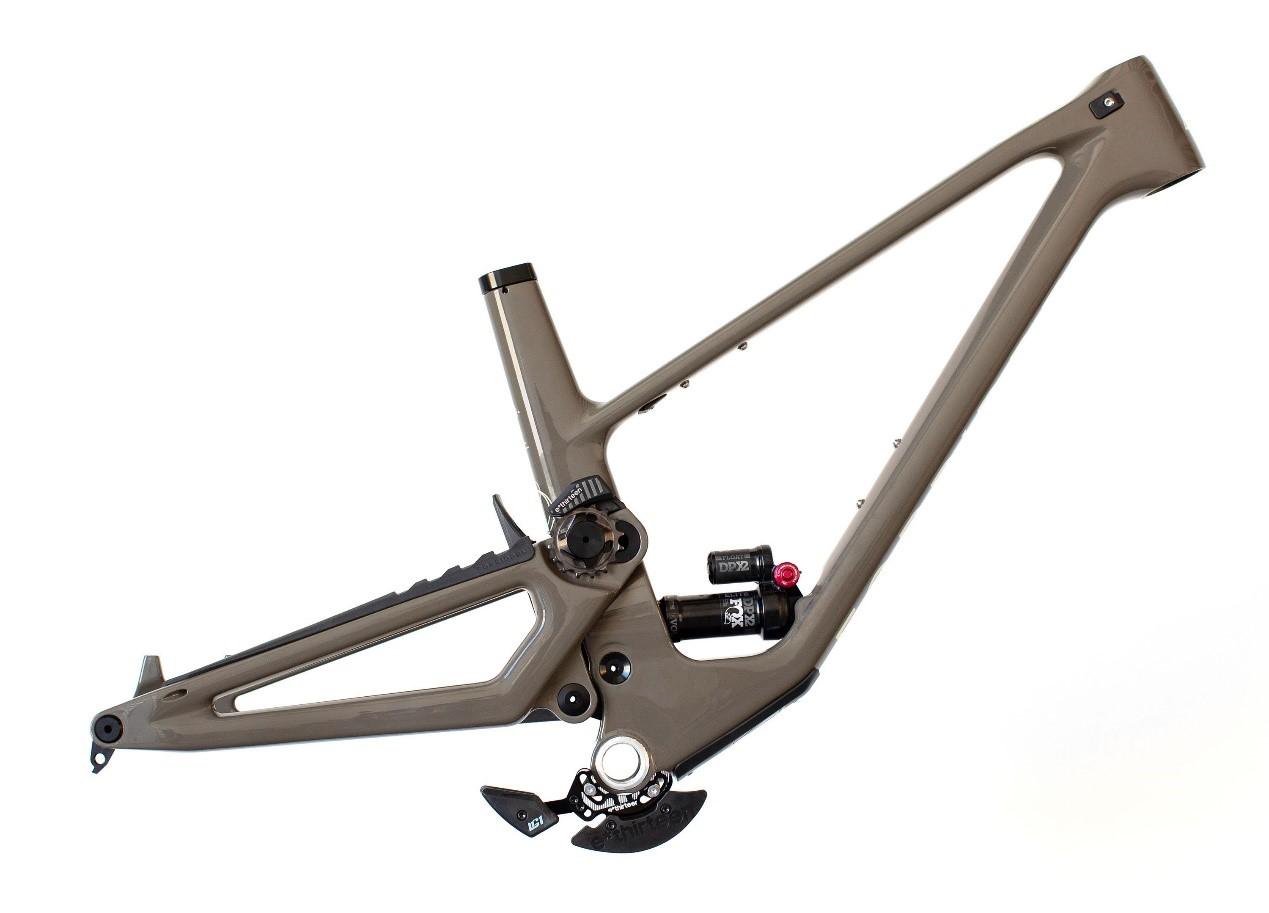
\includegraphics[scale=0.6]{高樞轉惰輪懸架.jpg} 
        %照片須放在和文檔相同之資料夾內
        \caption{高樞轉惰輪懸架} %有caption的圖才會編入目錄中
        \label{fig_High-Pivot Idler:scale} %此處的label相當於一個圖片的專屬標誌,目的是方便上下文的引用
    \end{figure}  
       \hspace*{\fill} \\
        \subsection{Twin-link suspension(雙連桿懸掛)}
        \hspace*{\fill} \\
         \fourteen {搖臂通過兩個搖桿連桿安裝在框架上,從而將搖臂連接到主機樞軸,通過擺臂或搖臂連桿之一來驅動衝擊。
         \hspace*{\fill} \\  
         雙連桿懸架將樞軸的數量從一增加到四個,可修改中心位置,進而改變行程不同點的懸架特性,參考產品為Ibis’ DW-link Suspension的Mojo HD5 Frame – 2020,如圖\ref{fig_Twin-link:scale}。}
     \begin{figure}[hbt!]
        \centering
        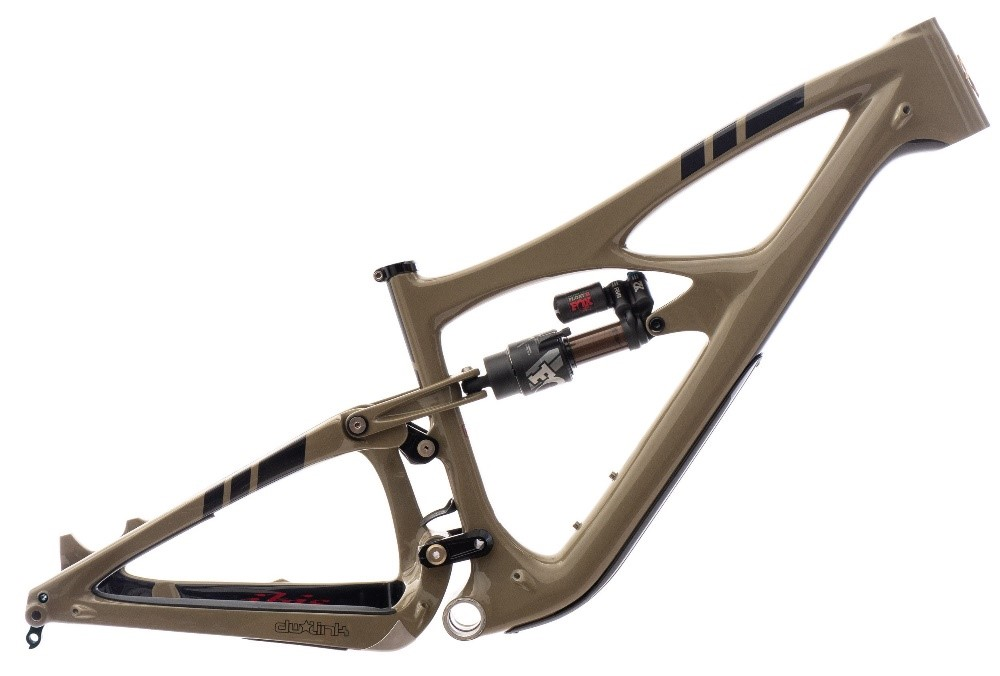
\includegraphics[scale=0.7]{雙連桿懸掛.jpg} 
        %照片須放在和文檔相同之資料夾內
        \caption{雙連桿懸掛} %有caption的圖才會編入目錄中
        \label{fig_Twin-link:scale} %此處的label相當於一個圖片的專屬標誌,目的是方便上下文的引用
    \end{figure}
    \newpage  
    	\hspace*{\fill} \\
        \subsection{Horst-link suspension(霍斯特鏈懸掛)}
        \hspace*{\fill} \\
         \fourteen {特性在於樞軸底端的鏈條,後軸則安裝在腳撐上增加了樞軸,其修改後的軸距繞即時中心旋轉,改變行進路線的位置,可在行進的不同階段優化防下蹲與上抬。
         \hspace*{\fill} \\  
雙連桿懸掛相比,霍斯特連桿系統的較長連桿通常會提供更平滑的曲線,產品為 Canyon Spectral的Izzo Pro Race 29,如圖\ref{fig_Horst-link:scale}。}
     
     \begin{figure}[hbt!]
        \centering
        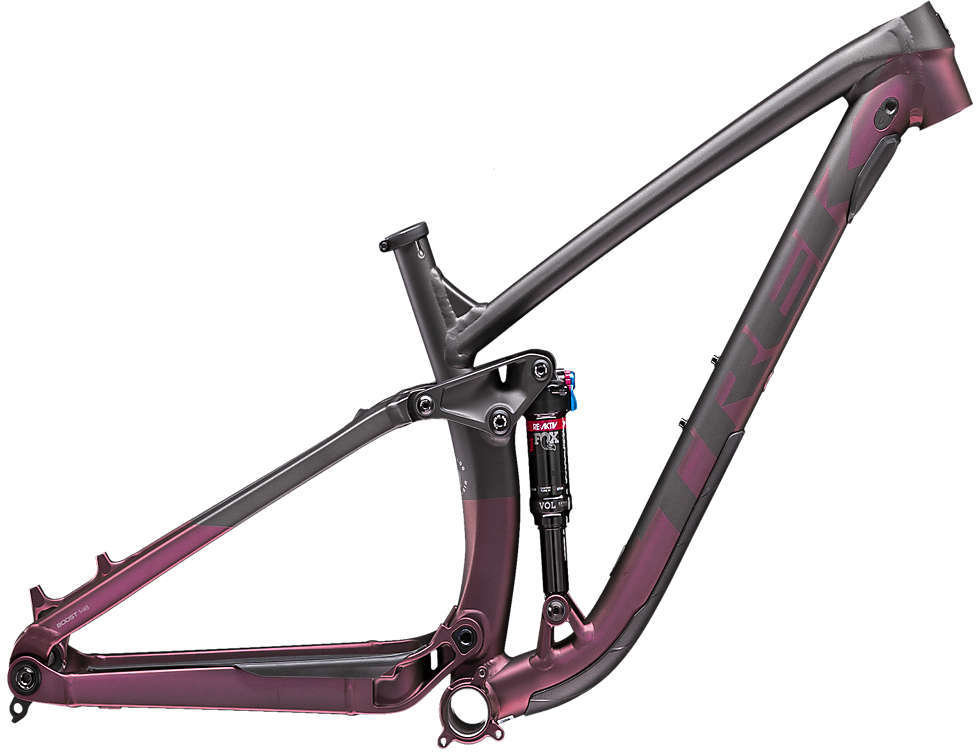
\includegraphics[scale=0.2]{霍斯特鏈懸掛2.jpg} 
        %照片須放在和文檔相同之資料夾內
        \caption{霍斯特鏈懸掛} %有caption的圖才會編入目錄中
        \label{fig_Horst-link:scale} %此處的label相當於一個圖片的專屬標誌,目的是方便上下文的引用
    \end{figure} 
    
      \chapter{Pyslvs-UI 套件介紹}
      \section{Pyslvs-UI 架構與原理}
       \fourteen{Pyslvs-UI是一套利用Python3與PyQt5建立的平面機構模擬與合成系統。機構模擬與合成的主要核心包括Python-Solvespace幾何約束求解程式庫、三角幾何函式程式庫(tinycadlib)、演算程式庫(ADesign)、幾何約束求解程式庫(bgfs)、類型合成程式庫(topologic)、數目合成程式庫(number)等。其中,ADesign演算程式庫內包含Real-coded Genetic Algorithm (RGA)、Differential Evolution(DE)與Firefly Algorithm (Firefly)等三種,用於平面機構尺寸合成演算}
       \begin{figure}[H]
        \centering
        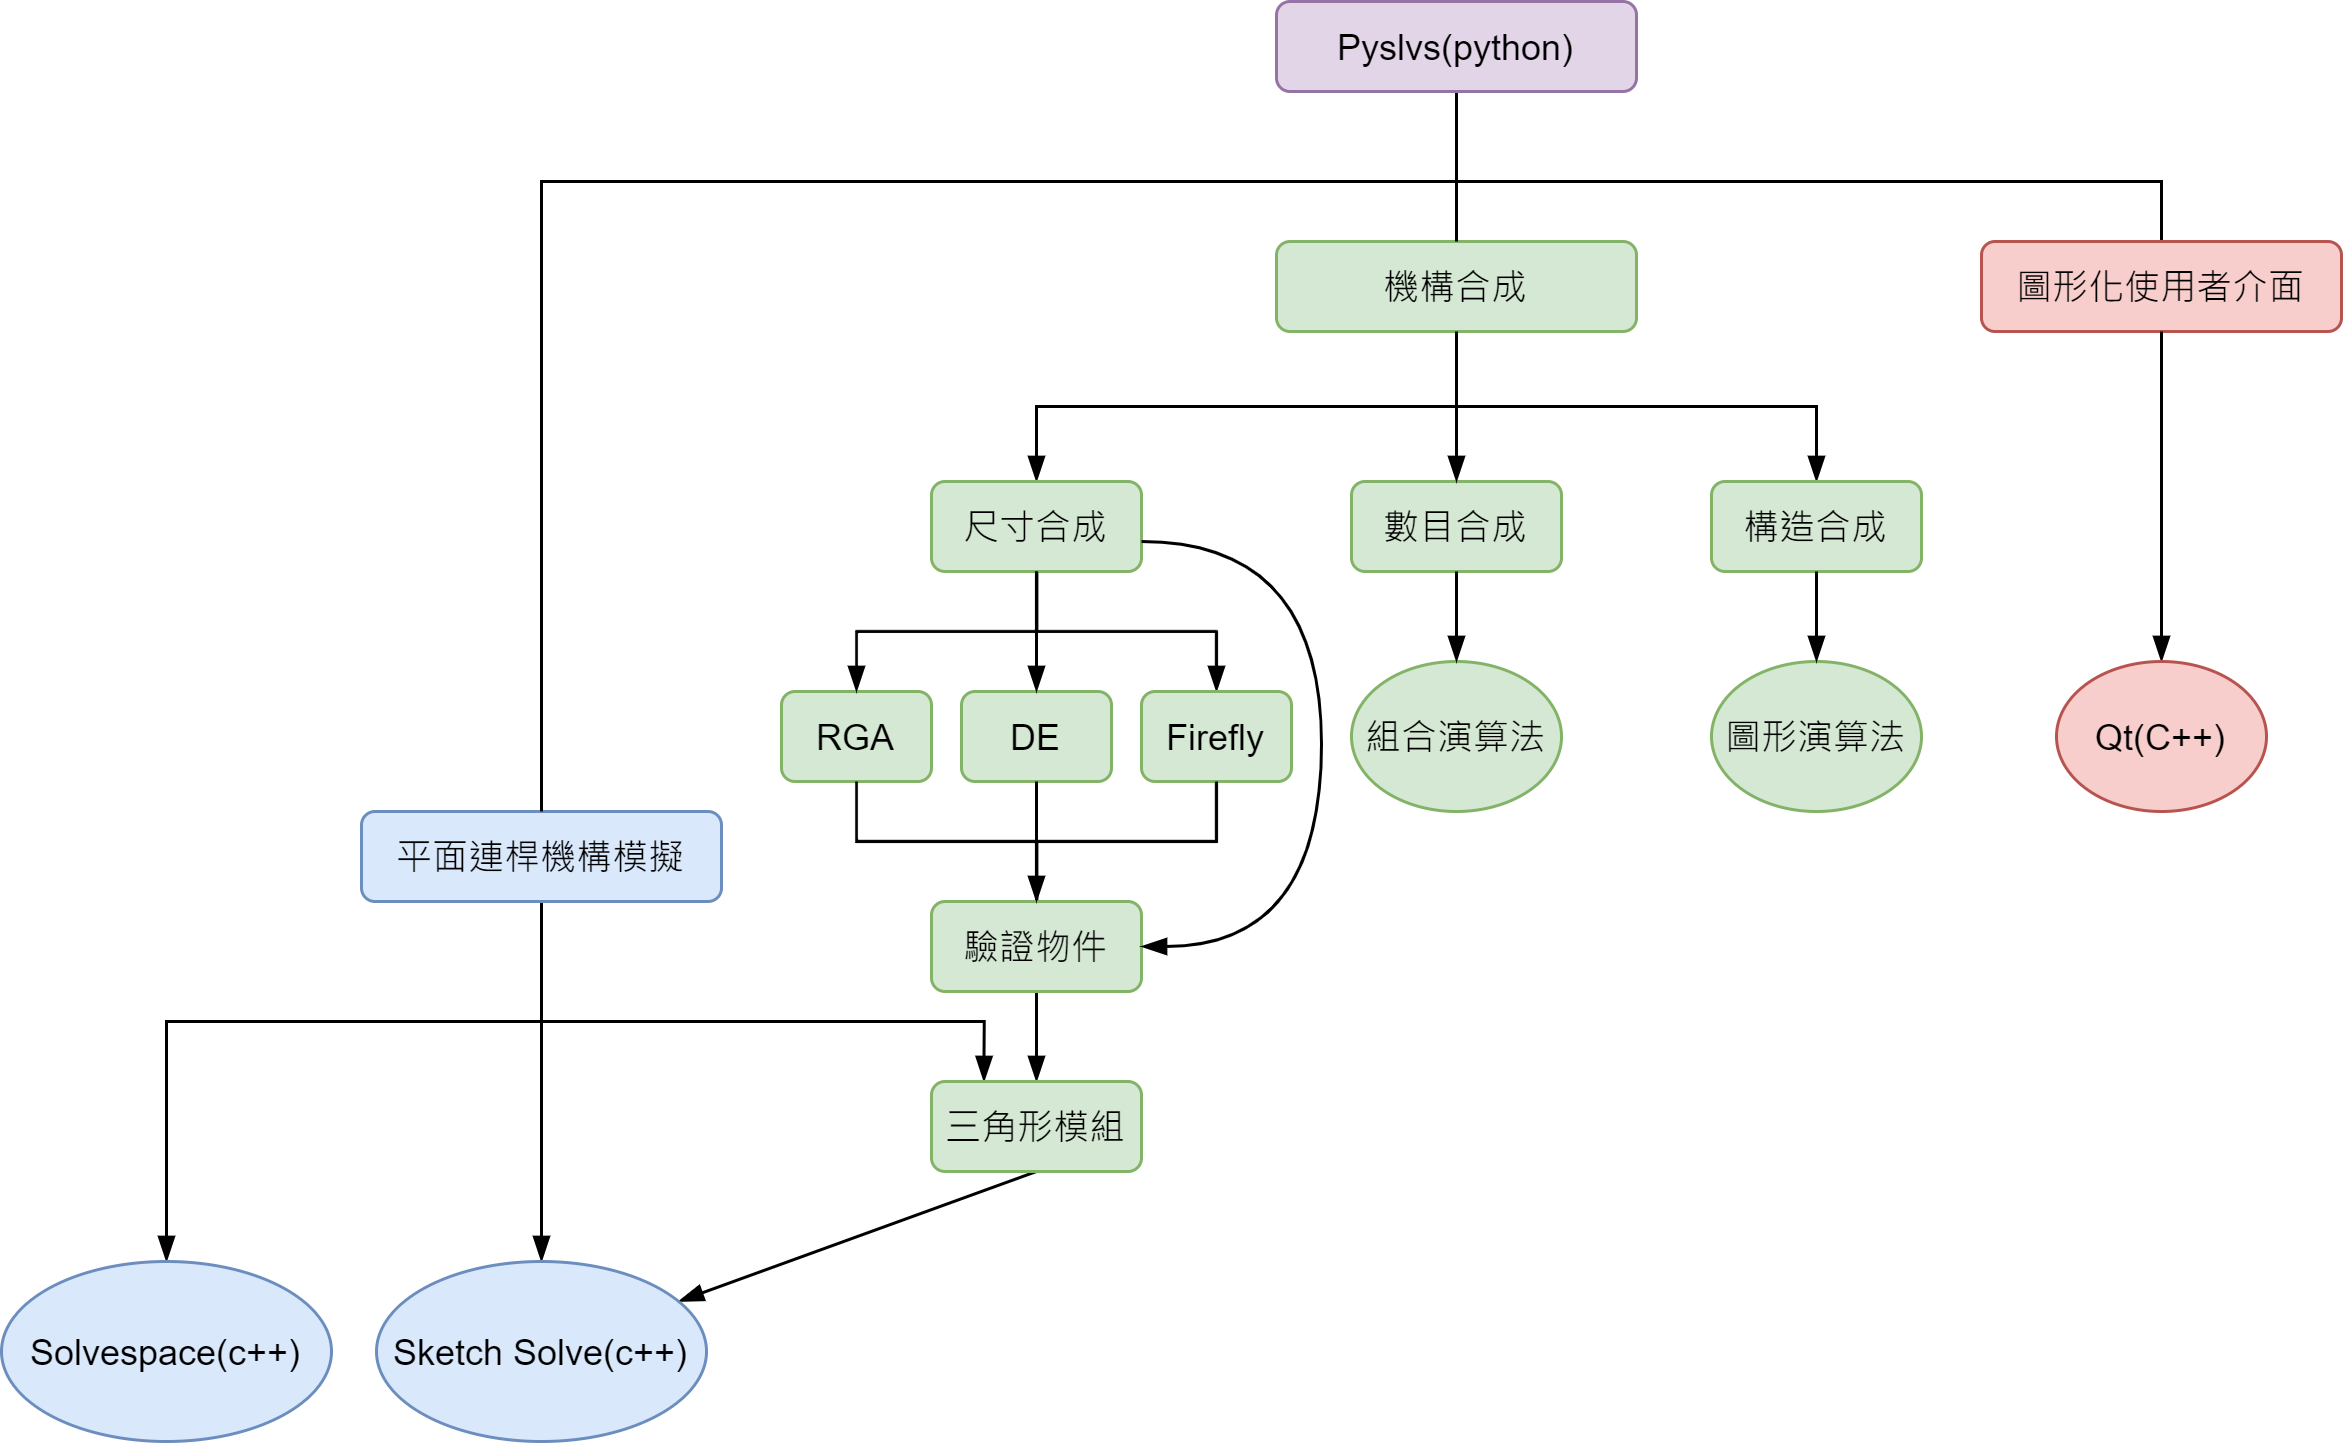
\includegraphics[scale=0.5]{Pyslvs-UI架構圖.png} 
        \caption{Pyslvs-UI架構圖} 
        \label{fig:scale}
    	\end{figure}
    	
    	
      \subsection{平面連桿機構模擬}
      \begin{itemize} 
      \item Solvespace:以C ++語言編寫的開放原始碼電腦輔助設計軟件,將幾何約束求解器分為實體與約束兩部份。其中,實體:表示每個圖形零件的幾何數據。約束: 表示圖形零件之間的關係。

		\begin{figure}[H]
        \centering
        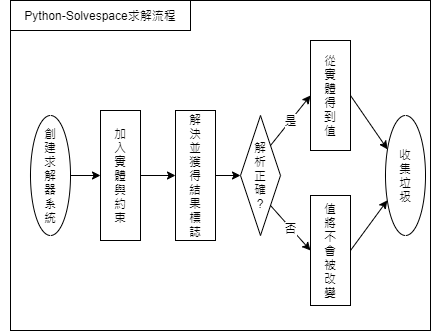
\includegraphics[scale=0.25]{Python-Solvespace求解流程.png} 
        \caption{Python-Solvespace流程圖} 
        \label{fig:scale}
    	\end{figure}
    	
      \item Sketch Solve:在BSD授權條款下,用C ++編寫的2D幾何求解器庫,原始碼僅使用表達式和函數來獲取答案。主要求解過程為:通過函數輸入創建約束對象,求解需要有參數列表、約束數據列表和步距精度,啟動BFGS算法後,參數將投影到每個實例,因此將更改值;若列表中沒有值,則該值將不會更改。
      	\end{itemize} 
      	
		\begin{figure}[H]
        \centering
        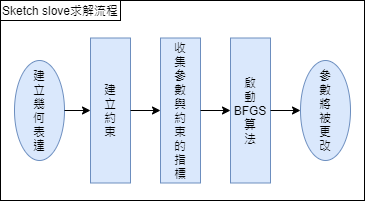
\includegraphics[scale=0.3]{Sketch slove.png} 
        \caption{Sketch slove流程圖} 
        \label{fig:scale}
    	\end{figure}
    	
      \fourteen{Cython是結合了Python和C語法的一種語言,使用者可以維持大部分的Python語法,而不需要大幅度調整主要的程式邏輯與演算法。}
      
      
      \subsection{平面連桿機構合成}
      \fourteen{進行機構設計與合成主要流程分為數目合成、構造合成、尺寸合成與運動學模擬,合成皆有其順序性存在,而運動學模擬則是進行分析前面的合成項目。}
      \begin{itemize} 
      \item 數目合成:用來決定其設計機構的桿數與接頭數,如四連桿、五連桿、六連桿等,然而當機構的桿數與接頭數越多的時候,其組合變化亦越多,將所有可能的運動鏈全部列出來。
      \item 構造合成:構造合成可分為以下幾個步驟
      \end{itemize} 
      \begin{enumerate}
      \item 確定自由度數:機構的獨立輸入數是根據其工作目的來決定,為已知條件。
      \item 選擇運動空間類型:必須根據設計規範、設計要求、設計限制來選擇
      \item 決定接頭類型:接頭類型必須根據工作目的、運動空間類型來決定,若無特殊考量,以取自由度為1的接頭為宜。
      \item 求出機件與接頭數目:當機構的運動空間類型與接頭類型確定後,即可根據式(3.1)或(3.2)求出機件數目N與接頭數目J
      \hspace*{\fill} \\
      
      \begin{equation}
      F_{p}=3\left ( N-1 \right )-\sum J_{i}C_{pi}
      \end{equation}  
      
      \begin{equation}
      F_{s}=6\left ( N-1 \right )-\sum J_{i}C_{si}
      \end{equation}  
      \item 合成機構構造目錄:針對每一個具N根機件與J個接頭的運動鏈,根據要求與限制,將機件與接頭類型其分別配置到適合的桿件與接頭上。
      \hspace*{\fill} \\
      \end{enumerate}
      \begin{itemize} 
      \item 尺寸合成:
      \end{itemize} 
      \fourteen {通過隨機變量生成具有路徑限制的機構,生成結構參數來自變數設定,也有其它算法選擇,程式內共包含三種算法:實數編碼遺傳算法、螢火蟲算法與差分進化演算法。}
      \begin{enumerate}
      \item {實數編碼遺傳算法:在遺傳演算法的演算過程中,將設計變數以實數數值表示,稱為實數編碼遺傳演算法(RGA),其演算流程如圖3.1}
      \begin{figure}[hbt!]
        \centering
        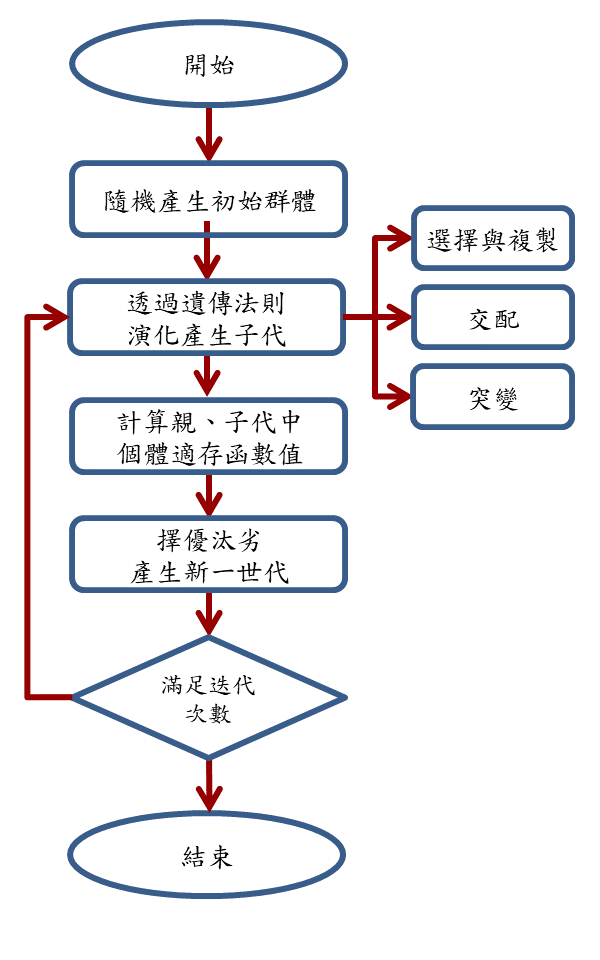
\includegraphics[scale=0.3]{實數編碼遺傳算法.png} 
        \caption{實數編碼遺傳算法流程圖}
        \label{fig:scale}
        \end{figure}
        
       \item {螢火蟲算法:其演算法是模擬螢火蟲離散的閃爍行為,算法將計算群體中螢火蟲的相對亮度和吸引度,並根據相對亮度決定螢火蟲的移動方向;更新螢火蟲的空間位置,對處在最佳位置的螢火蟲進行隨機移動;根據更新後螢火蟲位置,重新計算螢火蟲的亮度,最終輸出群體極值點和最優個體數值,演算流程如圖3.2。}
       
		\begin{figure}[hbt!]
        \centering
        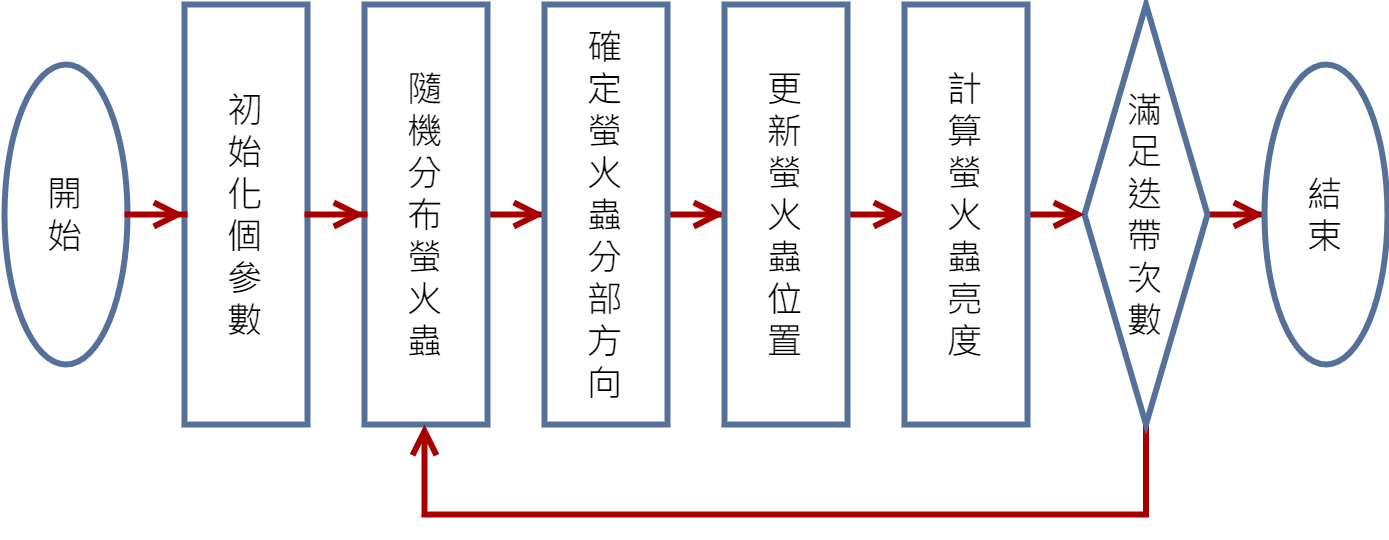
\includegraphics[scale=0.3]{螢火蟲算法.png} 
        \caption{螢火蟲算法流程圖}
        \label{fig:scale}
        \end{figure}
    \newpage   
       \item {差分進化演算法:是一種求解最佳化問題的進化演算法,其算法]]]原理採用對個體進行方向擾動,以達到對個體的函式值進行下降的目的,同其他進化演算法一樣,差分進化演算法不利用函式的梯度資訊,因此對函式的可導性甚至連續性沒有要求,適用性很強,演算流程如圖3.3。} 
                       
        \begin{figure}[hbt!]
        \centering
        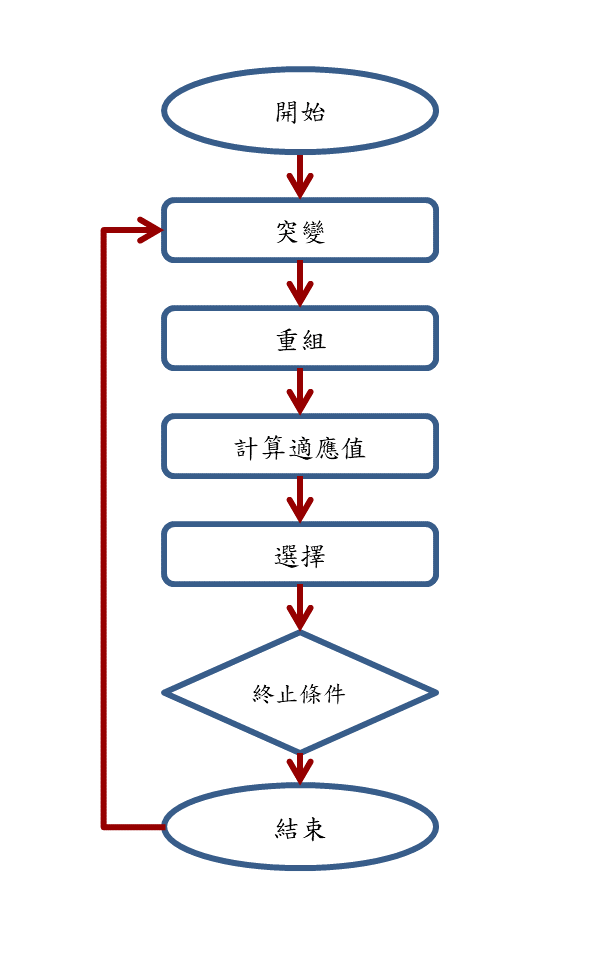
\includegraphics[scale=0.3]{差分進化演算法.png} 
        \caption{差分進化演算法流程圖}
        \label{fig:scale}
		\end{figure}
		
	\end{enumerate}
    \newpage
      \subsection{圖形化使用者介面}
      \begin{itemize}
      \item{PyQt}
      \end{itemize}
      \fourteen {Qt被廣泛應用於開發圖形化介面程式。主要特色為使用相同的程式碼皆可在支援的平台上執行與編譯,PyQt是Python語言的GUI編程解決方案之一,與Qt一樣是一個自由軟體,其API也與Qt類似,因此Qt的文件仍然可以應用於此,且與相同性質的軟體比較,PyQt的編程庫文件豐富許多。} 
      \begin{figure}[hbt!]
        \centering
        
\includegraphics[scale=0.1]{PyQt.png} 
        \caption{PyQt圖示}
        \label{fig:scale}
        \end{figure}
      \section{Pyslvs-UI 編譯}
       \lstset{language=Python, %設定語言
		basicstyle=\footnotesize, 
		frame=lines,
		caption={Python code}, %設定capion
		label={lst:example} %設定label
		}



\subsection{環境與安裝套件}
		\begin{itemize}
		\item 下載倉儲且安裝 3.0a6 版本的 Cython 模組
		\begin{lstlisting}[caption=下載倉儲安裝Cython]
https://github.com/mdecourse/ps2020.git
pip install cython==3.0a6
		\end{lstlisting}
		\end{itemize}

		\begin{itemize}
		\item 儲存檔案於倉儲中,以下為txt檔案中需安裝模組套件的名稱
		\begin{lstlisting}[caption=安裝模組套件]
importlib-metadata; python_version < '3.8'
requests
qtpy
pyqt5
ezdxf
numpy
matplotlib
openpyxl
lark-parser
pyyaml
h5py
qrcode
		\end{lstlisting}
		\end{itemize}
		
		\begin{itemize}
		\item 利用可攜下載txt檔中缺少的模組套件
		\begin{lstlisting}[caption=安裝模組套件指令]
pip install -r requirements.txt
		\end{lstlisting}
		\end{itemize}
		
		\begin{itemize}
		\item 套件安裝完成後進入pyslvs檔案,安裝setup.py檔
		\begin{lstlisting}[caption=安裝步驟]
cd ps2020/pyslvs..
python setup.py install
		\end{lstlisting}
		\end{itemize}
		
		\begin{itemize}
		\item 回到ps2020根目錄再次下載安裝setup.py檔
		\begin{lstlisting}[caption=安裝步驟]
cd ..
python setup.py install
		\end{lstlisting}
		\end{itemize}
		
		\begin{itemize}
		\item {確認成功安裝在ps2020根目錄中,打pyslvs可看見畫面即為編譯成功,如圖\ref{fig_pyslvs:scale}}
      \begin{figure}[hbt!]
        \centering
        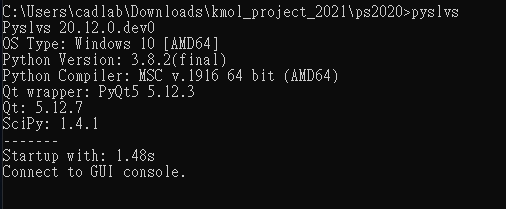
\includegraphics[scale=0.6]{輸入pyslvs指令.PNG}
        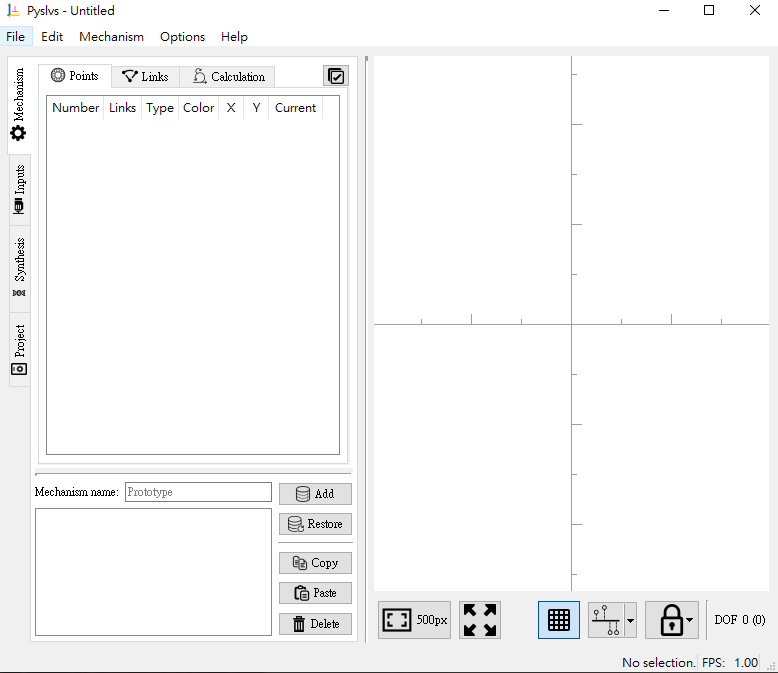
\includegraphics[scale=0.5]{編譯成功畫面.png}
        \caption{編譯成功畫面}
        \label{fig_pyslvs:scale} 
    	\end{figure}
		\end{itemize}
      

      
    
      \section{Pyslvs-UI 範例}
		\subsection{曲柄滑塊機構}
       \hspace*{\fill} \\
       \fourteen {主要以6個連桿、7個接頭,4個雙接頭連桿、1個三接頭連桿所構成,如圖\ref{fig_Crank Lifter:scale},由四連桿機構衍伸而來多樣性運動型態、軌跡,可滿足一般運動需求,常用於汽車工業中加速與製動,從踏板的輸入到化油器、製動缸、自行車剎車都廣泛運用在其中,如圖\ref{fig_Crank Lifter1:scale}。}\\
     \begin{figure}[H]
        \centering
        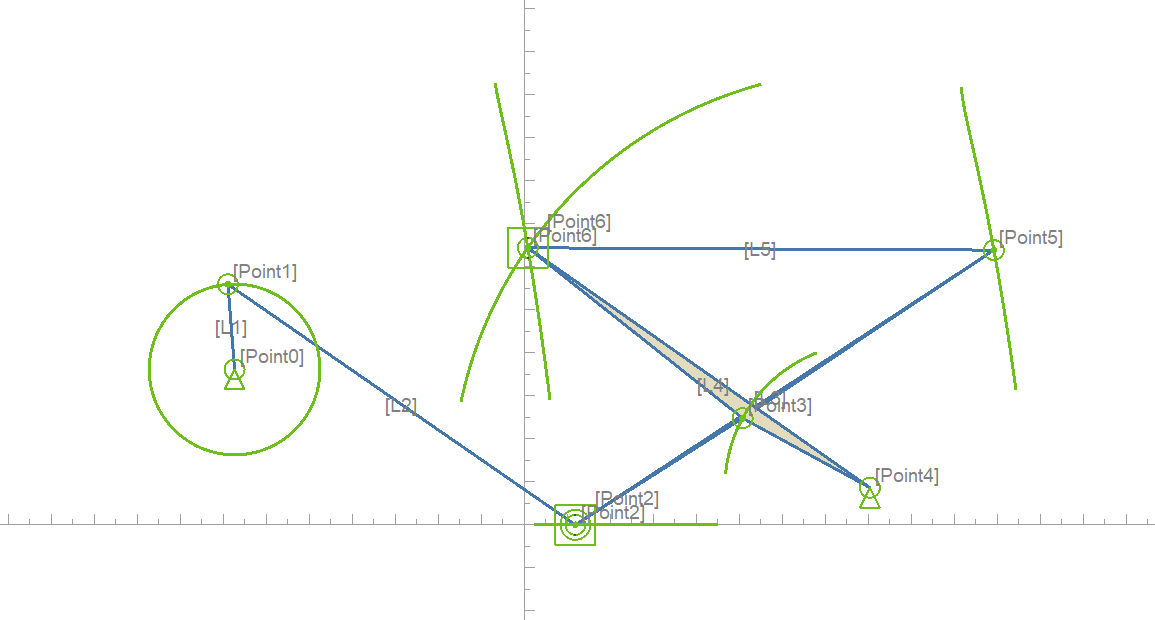
\includegraphics[scale=0.5]{曲柄滑塊機構.png} 
        %照片須放在和文檔相同之資料夾內
        \caption{曲柄滑塊機構} %有caption的圖才會編入目錄中
        \label{fig_Crank Lifter:scale} %此處的label相當於一個圖片的專屬標誌,目的是方便上下文的引用
    \end{figure}
    \begin{figure}[H]
        \centering
        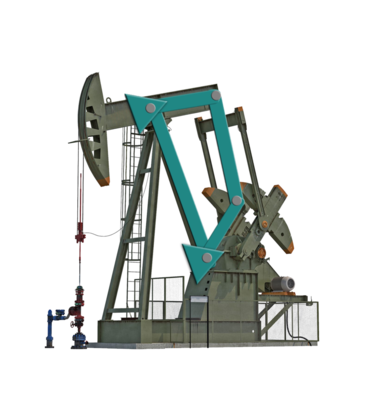
\includegraphics[scale=0.6]{曲柄滑塊機構運用範圍.png} 
        %照片須放在和文檔相同之資料夾內
        \caption{曲柄滑塊機構運用範圍} %有caption的圖才會編入目錄中
        \label{fig_Crank Lifter1:scale} %此處的label相當於一個圖片的專屬標誌,目的是方便上下文的引用
    \end{figure}
    
    
       \hspace*{\fill} \\
       \subsection{曲柄搖桿機構}
       \hspace*{\fill} \\        
        \fourteen {為4個連桿、5個接頭,2個雙接頭連桿、1個三接頭連桿所組成,如圖\ref{fig_Crank Rocker:scale},曲柄旋轉運動透過連接桿轉換至搖桿的搖擺運動,此四連桿機構構造最簡單也最常在生活周遭出現,如:老虎鉗、雷達調整機構、縫紉機腳踏機構、鋼材輸送機,如圖\ref{fig_Crank Rocker1:scale}。}
     \begin{figure}[H]
        \centering
        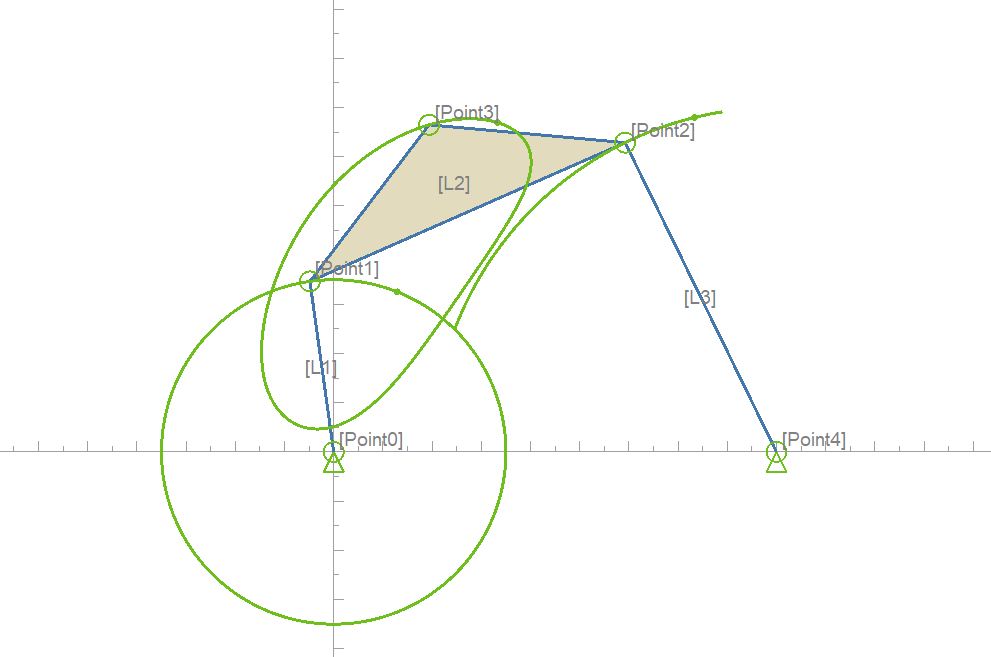
\includegraphics[scale=0.5]{曲柄搖桿機構.png} 
        %照片須放在和文檔相同之資料夾內
        \caption{曲柄搖桿機構} %有caption的圖才會編入目錄中
        \label{fig_Crank Rocker:scale} %此處的label相當於一個圖片的專屬標誌,目的是方便上下文的引用
    \end{figure}
    \begin{figure}[H]
        \centering
        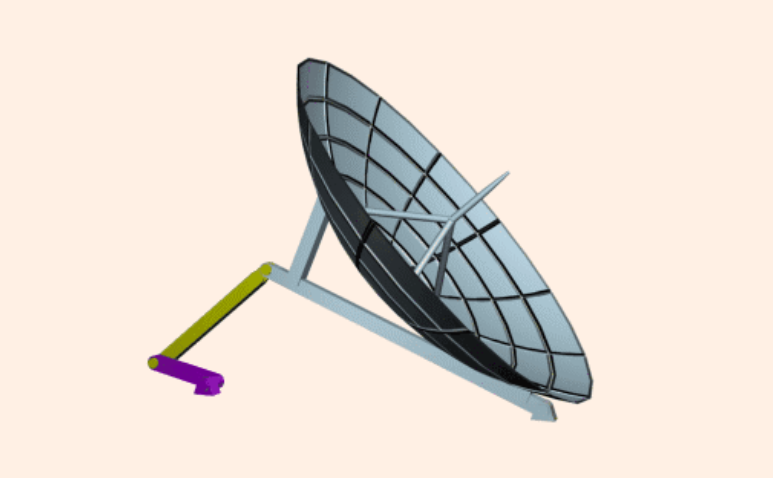
\includegraphics[scale=0.6]{曲柄搖桿機構範例.png} 
        %照片須放在和文檔相同之資料夾內
        \caption{曲柄搖桿機構範例} %有caption的圖才會編入目錄中
        \label{fig_Crank Rocker1:scale} %此處的label相當於一個圖片的專屬標誌,目的是方便上下文的引用
    \end{figure}
    
    
    	\hspace*{\fill} \\
       \subsection{史蒂芬生機構}
       \hspace*{\fill} \\        
        \fourteen {為6個連桿、7個接頭,3個雙接頭連桿、2個三接頭連桿所組成,使三接頭連桿作為固定桿,其中一雙接頭連桿作曲柄運動,其餘桿件與三接頭連桿一起做搖擺運動,如圖\ref{fig_Stephenson:scale},此機構僅次於四連桿組的重要單自由度連桿機構也稱作複合連桿組機構,常用於自動化夾緊機構、越野摩托車後懸吊系統,如圖\ref{fig_Stephenson1:scale}。
}
     \begin{figure}[H]
        \centering
        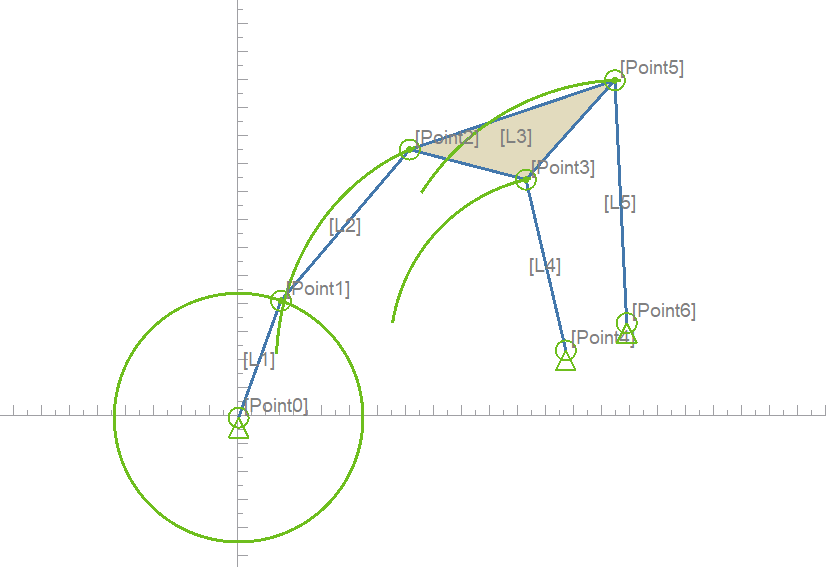
\includegraphics[scale=0.5]{史蒂芬生機構作動.png} 
        %照片須放在和文檔相同之資料夾內
        \caption{史蒂芬生機構作動} %有caption的圖才會編入目錄中
        \label{fig_Stephenson:scale} %此處的label相當於一個圖片的專屬標誌,目的是方便上下文的引用
    \end{figure}
    \begin{figure}[H]
        \centering
        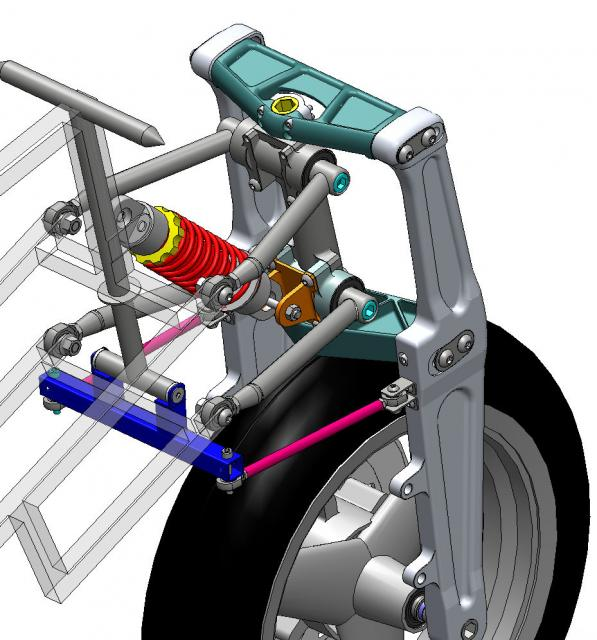
\includegraphics[scale=0.4]{史蒂芬生機構範例.jpg} 
        %照片須放在和文檔相同之資料夾內
        \caption{史蒂芬生機構範例} %有caption的圖才會編入目錄中
        \label{fig_Stephenson1:scale} %此處的label相當於一個圖片的專屬標誌,目的是方便上下文的引用
    \end{figure}
    
    
    \hspace*{\fill} \\
       \subsection{瓦特氏運動機構}
       \hspace*{\fill} \\        
        \fourteen {由6個連桿、7個接頭,4個雙接頭連桿、1個三接頭連桿構成,本身機械鏈構型為上下左右對稱,使三接頭桿為固定桿另其中一支雙接頭桿為曲柄作旋轉運動,其他桿件則是搖擺運動,如圖\ref{fig_Watt:scale},常用於自動化平台舉高移送機構、自動化包裹移送機構、磨耗測試裝置、飛機起落收放機構,如圖\ref{fig_Watt1:scale}。}
     \begin{figure}[H]
        \centering
        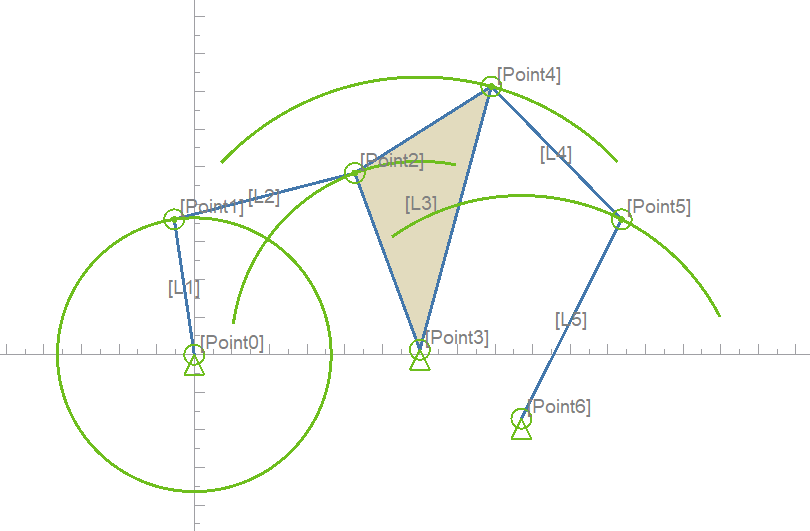
\includegraphics[scale=0.5]{瓦特氏運動機構.png} 
        %照片須放在和文檔相同之資料夾內
        \caption{瓦特氏運動機構} %有caption的圖才會編入目錄中
        \label{fig_Watt:scale} %此處的label相當於一個圖片的專屬標誌,目的是方便上下文的引用
    \end{figure}
    \begin{figure}[H]
        \centering
        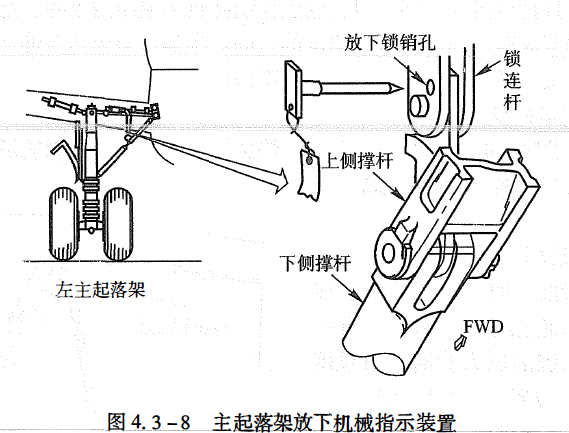
\includegraphics[scale=0.6]{瓦特氏運動機構飛機起落收放.png} 
        %照片須放在和文檔相同之資料夾內
        \caption{瓦特氏運動機構飛機起落收放} %有caption的圖才會編入目錄中
        \label{fig_Watt1:scale} %此處的label相當於一個圖片的專屬標誌,目的是方便上下文的引用
    \end{figure}
    
    
  	 \hspace*{\fill} \\
       \subsection{二段式提球機構}
       \hspace*{\fill} \\        
        \fourteen {由兩個史蒂芬生 (Stephenson) 機構衍伸出來,將機構融合調整位置後為10個連桿、14個接頭,8個雙接頭連桿、1個三接頭連桿所組成,如圖\ref{fig_Double Ball Lifter:scale},便於機構執行時接近置球點底部,將球提起並筆直向上提升與下一個提球機構交會完成傳接行程,常運用在搖臂式發球機上,如圖\ref{fig_Double Ball Lifter1:scale}。}
    \begin{figure}[H]
        \centering
        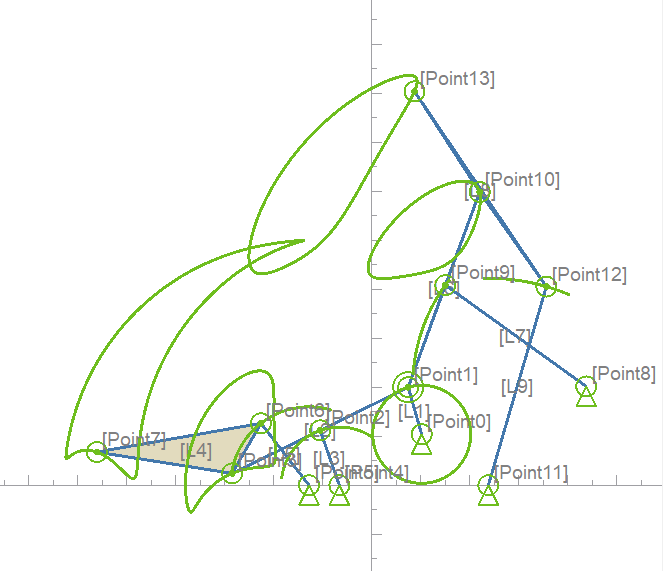
\includegraphics[scale=0.6]{雙球升降器.png} 
        %照片須放在和文檔相同之資料夾內
        \caption{雙球升降器} %有caption的圖才會編入目錄中
        \label{fig_Double Ball Lifter:scale} %此處的label相當於一個圖片的專屬標誌,目的是方便上下文的引用
    \end{figure}
    \begin{figure}[H]
        \centering
        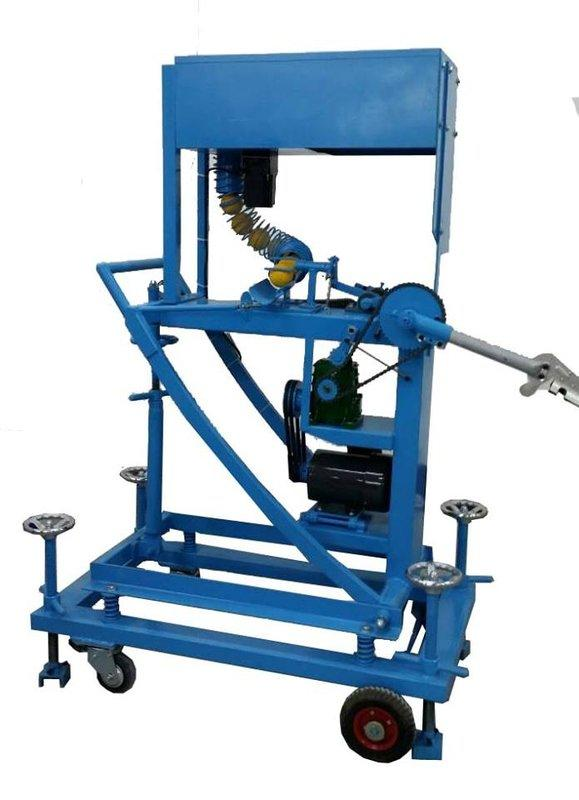
\includegraphics[scale=0.3]{搖臂式發球機.jpg} 
        %照片須放在和文檔相同之資料夾內
        \caption{搖臂式發球機} %有caption的圖才會編入目錄中
        \label{fig_Double Ball Lifter1:scale} %此處的label相當於一個圖片的專屬標誌,目的是方便上下文的引用
    \end{figure}
        \chapter{登山車避震機構}
      \section{避震機構合成}
      \subsection{差分進化演算法}
      \hspace*{\fill} \\
      \fourteen \quad {差分進化演算法\textrm{(Differential Evolution Algorithm)}概念是以向量為基礎,透過母體間的個體差異性,並以隨機搜尋方式將差異向量加上其中之個體中,並透過突變(Mutation)、重組(Recombination)、選擇(Selection)三個步驟進行演化,而透過迭代不斷地進行運算,並觀察個體是否能在搜尋解空間找到最佳解,該流程圖如圖\ref{fig_DEflow:scale}所示。}\\
	        
      \begin{figure}[hbt!]
        \centering
        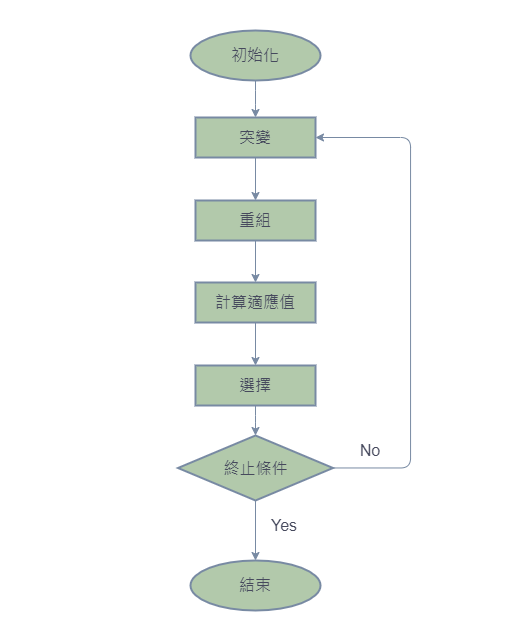
\includegraphics[scale=0.6]{DEflow.png}
        \caption{差分進化演算法流程圖}
        \label{fig_DEflow:scale}
    	\end{figure}
      
      \newpage
      \begin{enumerate}
      \item{\fourteen {初始化(Initialization):設定初始參數值及隨機產生介於上下限值以內的變數。}
      \begin{equation*}
      x_{n,i} = x_{n,i}^{L}+rand()*(x_{n,i}^{U}- x_{n,i}^{L})
	\qquad
i = 1,2,3,...D \ and \ n = 1,2,3,...N
	  \end{equation*}
	  $x_{i}^{L}$: 變數$x_{i}$的下限值
	  \hspace*{\fill} \\
	  \hspace*{\fill} \\
	  $x_{i}^{U}$: 變數$x_{i}$的上限值
	  }
	      
      \item{\fourteen {突變(Mutation):隨機從母體中選取三個目標向量並透過突變權重因子(weight factor)結合而得一合成向量(donor vector)。}
      \begin{equation*}
      v_{n}^{g+1} = x_{r1n}^{g}+F(x_{r2n}^{g}- x_{r3n}^{g})
      \end{equation*}
      $v_{n}^{g+1}$: 合成向量
      \hspace*{\fill} \\
	  \hspace*{\fill} \\
	  F: 權重因子
      }\\
      
      \item{\fourteen {重組(Recombination):經過前一突變步驟產生的合成向量,將利用條件式與挑選中的目標向量 $x_{n,i}^{g}$作一結合重組,並於重組後得到一新的試驗向量(Trial Vector)$u_{n,i}^{g+1}$。}
	  \begin{equation*}
	  u_{n,i}^{g+1} = 
\left\{\begin{matrix}
 & v_{n,i}^{g+1} & if \ rand() \leq C_{p} \\ 
 & x_{n,i}^{g} & if \ rand() > C_{p}
\end{matrix}\right.
\qquad i = 1,2,3,...D \ and \ n = 1,2,3,...N
	  \end{equation*}
	  $I_{rand}$: [1,D]之間的隨機整數
      \hspace*{\fill} \\
	  \hspace*{\fill} \\	
	  $C_{p}$: 重組的可能性,其數值在[0,1]之間}\\
	  
	\item{\fourteen {選擇(Selection):選擇階段主要執行方式為藉由計算適應值來評估其該選擇試驗向量亦或是原始的目標向量進入下一迭代,成為此代演化過後的子代。}}  
	  \begin{equation*}
	  x_{n}^{g+1} = 
\left\{\begin{matrix}
 & u_{n,i}^{g+1}  & if \ f(u_{n}^{g+1} < f(x_{n}^{g})) \\ 
 & x_{n}^{g} & otherwise
\end{matrix}\right.
\qquad n = 1,2,3,...N
	  \end{equation*}
      \end{enumerate}
      
      \subsection{適應性函數}
	  \quad \fourteen {機構合成設計需求為騎乘姿勢改變時或遇到顛頗不整的路時仍能保持整體的平衡,即Anti-squat及Anti-rise的數值能在100\%附近,而上述合成需求之適應函數可表示為}      
      
      \begin{equation}
      h_{2} = r_{of}\left (\frac{r_{ppy}-IFC_{y}}{r_{ppx}-IFC_{x}}\right ) + \left[ r_{ppy}-r_{ppx}\left( \frac{r_{ppy}-IFC_{y}}{r_{ppx}-IFC_{x}} \right) \right]
      \end{equation}  
      \hspace*{\fill} \\
      
      \fourteen {其中}
      \begin{equation}
      IFC_{x} = \frac{\left[ P_{2y} - \left( \frac{P_{2y} - IC_{y}}{P_{2x} - IC_{x}} \right )P_{2x} - otl_{b} \right ]}{\frac{P_{2y} - IC_{y}}{P_{2x} - IC_{x}}-otl_{a}}
      \end{equation}
      \hspace*{\fill} \\
      

      \begin{flushleft}
      \begin{equation}
      IFC_{y} = otl_{a} \cdot \left( IFC_{x} \right ) + otl_{b}
      \end{equation}
      \end{flushleft}
      \hspace*{\fill} \\
      
      \begin{equation}
      IC_{x} = \frac{P_{3y} - \left [ \frac {(P_{3y} - P_{4y})P_{3x}}{P_{3x}-P_{4x}} \right ]}{\frac{P_{1y}}{P_{1x}}-\left ( \frac{P_{3y} - P_{4y}}{P_{3x}-P_{4x}} \right )}
      \end{equation}
      \hspace*{\fill} \\
      
      \begin{equation}
      IC_{y} = \left ( \frac{P_{1y}}{P_{1x}} \right ) IC_{x}
      \end{equation}
      \hspace*{\fill} \\
      
      \fourteen {
      	\begin{flushleft}
      	$r_{ppx}$: 後輪與地面接觸點到座標原點的x座標
      	\\
      	\hspace*{\fill} \\
      	$r_{ppy}$: 後輪與地面接觸點到座標原點的y座標
      	\\
      	\hspace*{\fill} \\
      	$P_{nx}$: 點n的x座標
      	\\
      	\hspace*{\fill} \\
      	$P_{ny}$: 點n的y座標
      	\\
      	\hspace*{\fill} \\
      	$IC_{x}$: 瞬時中心到座標原點的x座標
      	\\
      	\hspace*{\fill} \\
      	$IC_{y}$: 瞬時中心到座標原點的y座標
      	\\
      	\hspace*{\fill} \\
      	$IFC_{x}$: 瞬時力量中心到座標原點的x座標
      	\\
      	\hspace*{\fill} \\
      	$IFC_{y}$: 瞬時力量中心到座標原點的y座標
      	\\
      	\hspace*{\fill} \\
      	$r_{of}$: 座標原點到前輪樞紐的水平距離
      	\end{flushleft}
      	}
      	
      \hspace*{\fill} \\
      \section{避震機構評量}
      \subsection{Anti-squat}
      \fourteen {當加速時因不同騎乘姿勢導致的重心位置變化而產生的力量轉移會讓懸架受壓縮力,而Anti-squat即為抵抗此後沉的能力。}
       \begin{itemize}
       \item > 100\%: 表示足以抵抗後沉的力量,而超過的力量將會變成拉伸力
       \item 100\%: 表示完全平衡了負載,即懸吊沒受到壓縮力或拉伸力
       \item 0~100\%: 表示部分後沉力量被抵抗
       \item < 0\%: 表示所有的後沉力量皆無被抵抗
       \end{itemize}
       
     \begin{figure}[hbt!]
       \centering
       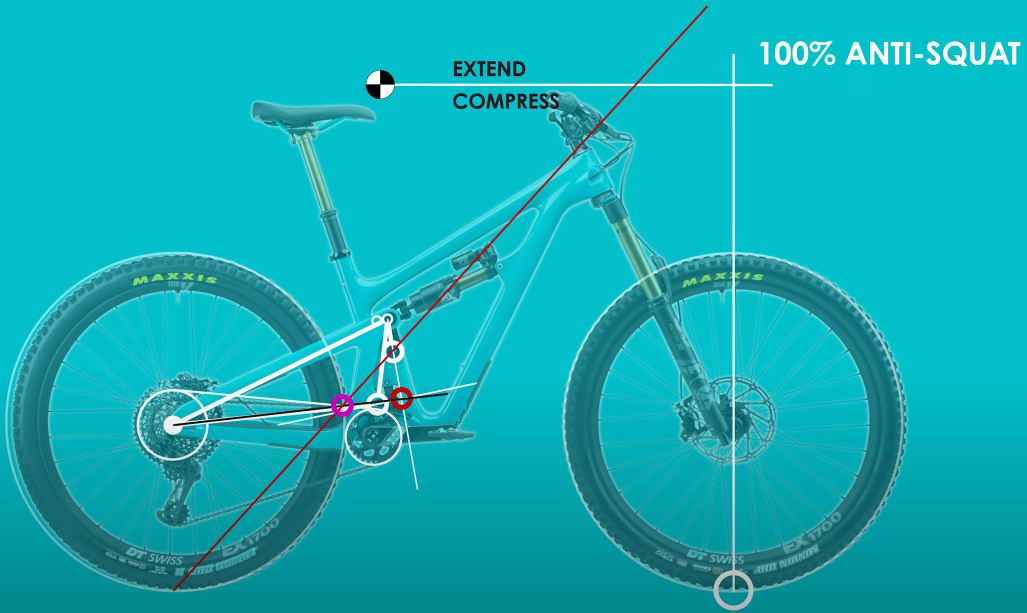
\includegraphics[scale=0.4]{anti-squat.PNG}
       \caption{Anti-squat}
       \label{fig_anti-squat:scale}
    \end{figure}
       
       \hspace*{\fill} \\
       \subsection{Anti-rise}
       \fourteen {在剎車的時候因為力量轉移的關係導致後輪產生升起的情況,而Anti-rise即為抵抗此後升現象的能力。}
       \begin{itemize}
       \item > 100\%: 表示足以抵抗後升的力量,而超過的力量將會變成壓縮力
       \item 100\%: 表示完全抵抗了剎車產生的後升現象
       \item 0~100\%: 表示部分後升力量被抵抗
       \item < 0\%: 表示所有的後升力量皆無被抵抗
       \end{itemize}
	\begin{figure}[hbt!]
       \centering
       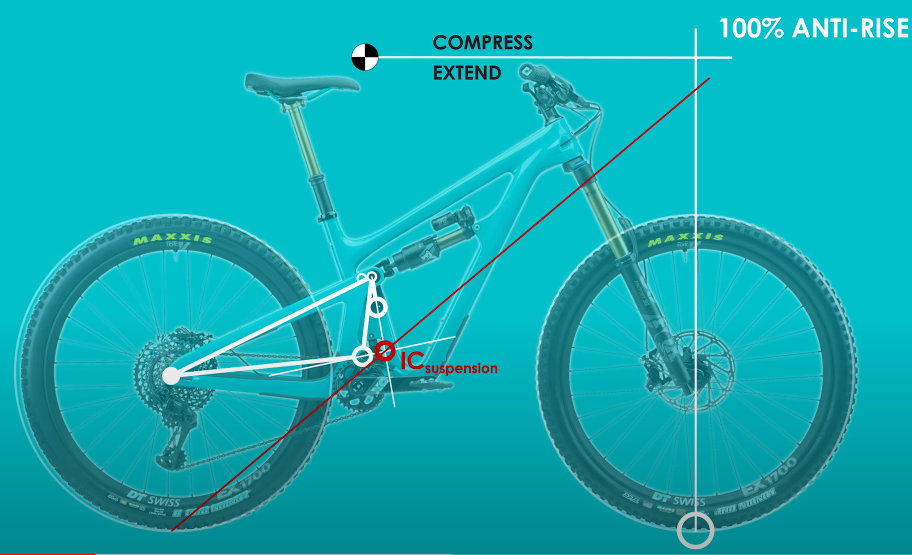
\includegraphics[scale=0.45]{anti-rise.PNG}
       \caption{Anti-rise}
       \label{fig_anti-rise:scale}
    \end{figure}
       
       
       \hspace*{\fill} \\
       \subsection{Leverage Ratio}
       \fourteen {Leverage ratio是避震器壓縮量和後輪行程的比值,當較大的槓桿比率會對避震器產生較大的衝擊,而在騎乘時對於地形變化的感受度較不敏感,相反地較小的槓桿比率對於地形的敏感度較高。其計算方式如下所示。}
       \hspace*{\fill} \\
       \begin{equation}
       Leverage\, Ratio = \frac{wheel\,travel}{stroke}
       \end{equation}

       
       \begin{figure}[hbt!]
        \centering
        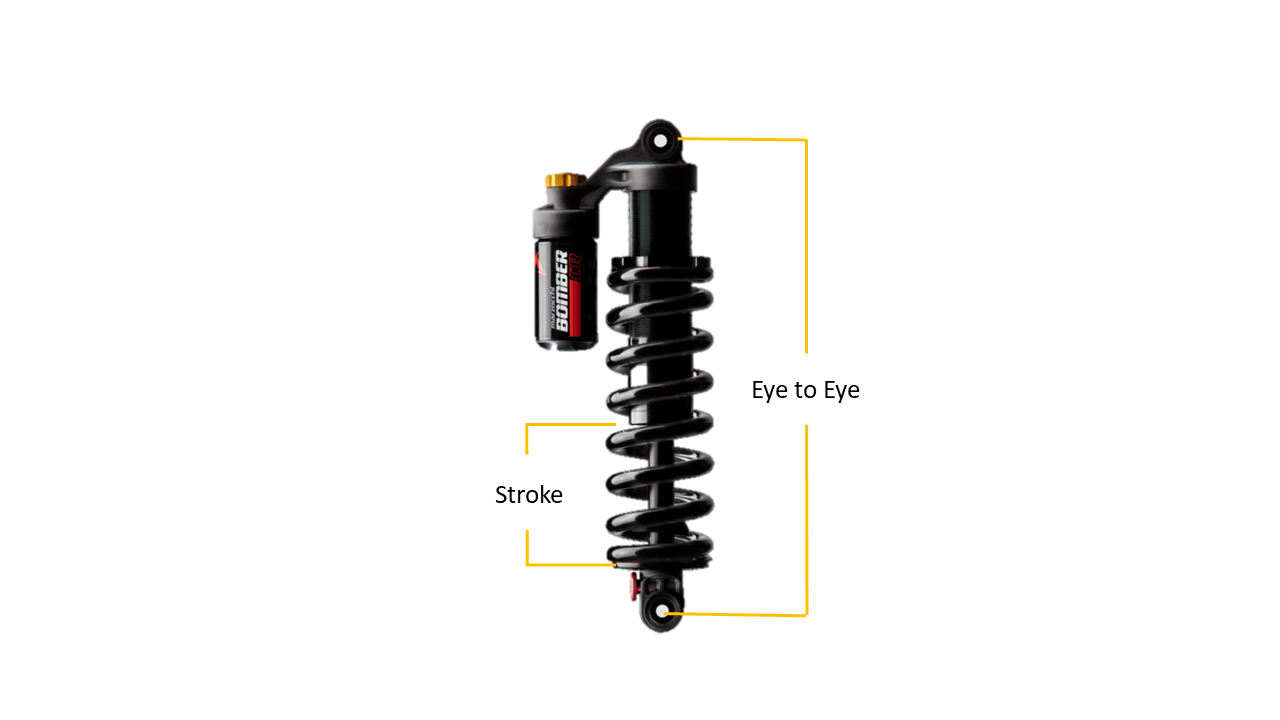
\includegraphics[scale=0.4]{stroke.png}
        \caption{避震器}
        \label{fig_stroke:scale}
    	\end{figure}
       
       
       \section{避震機構分析範例}
       \fourteen {此小節會將4.1節所得到的結果並配合4.2節所介紹的評比標準進行討論以檢驗是否得到最佳的尺寸。}
		\begin{figure}[hbt!]
        \centering
        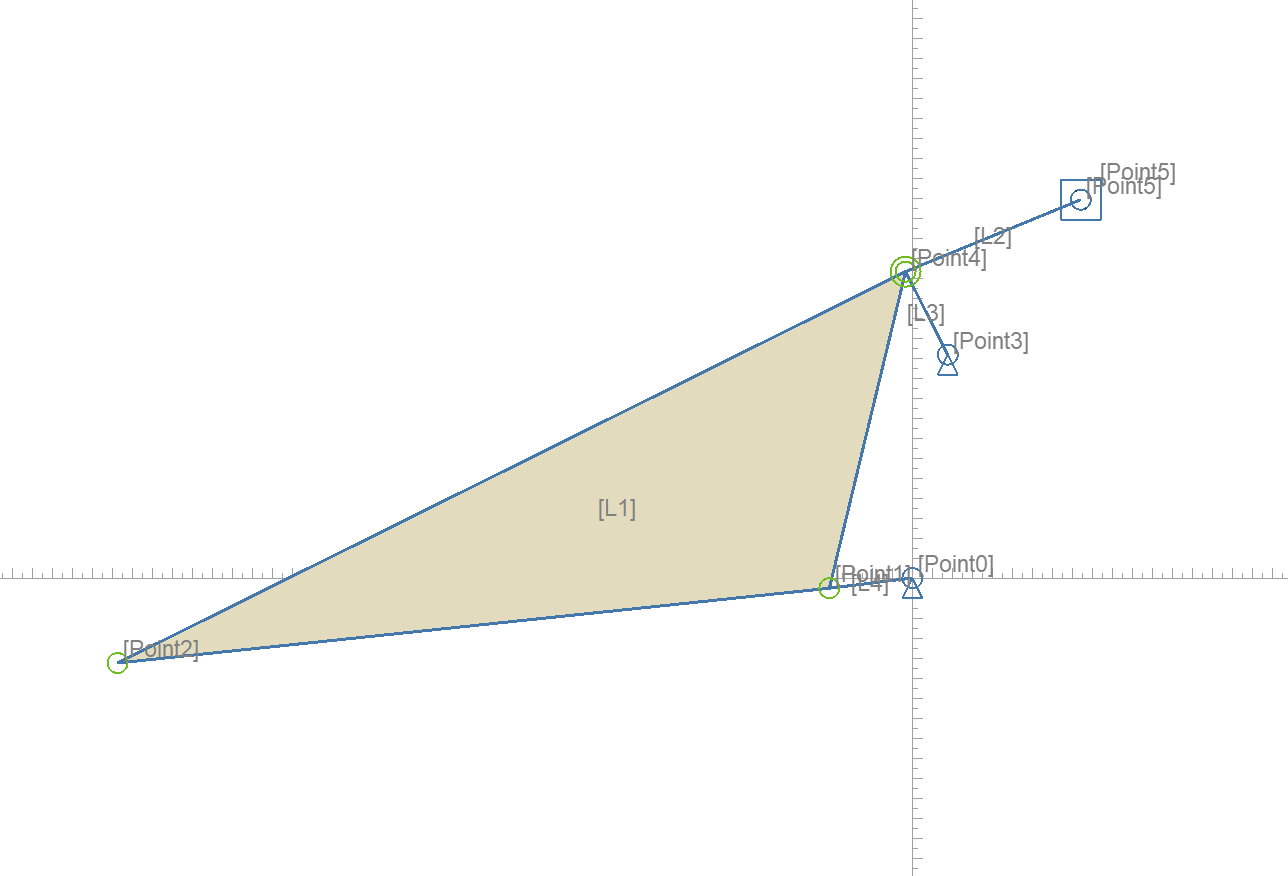
\includegraphics[scale=0.4]{Firebird_mechanism.png}
        \caption{合成所得之機構}
        \label{fig_Firebird_mechanism:scale}
    	\end{figure}
		
		\newpage
		\begin{flushleft}
	    \fourteen {圖\ref{fig_antisquat_x-:scale}為Point4 在x座標往負x方向移動時所得到Anti-squat評比結果,由該圖可知當Point4越往負x方向移動時所得到的結果會越偏離100\%。}
	    \end{flushleft}
      \begin{figure}[hbt!]
        \centering
        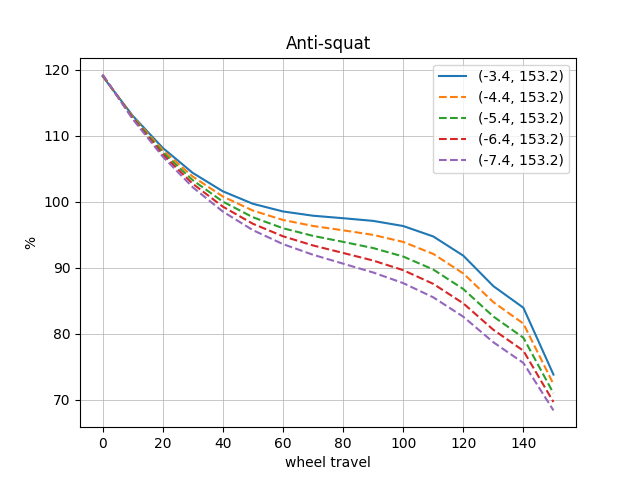
\includegraphics[scale=0.6]{anti-squat_x-.png}
        \caption{Anti-squat x座標減少}
        \label{fig_antisquat_x-:scale}
    	\end{figure}
    	
    	\begin{flushleft}
    	\fourteen {圖\ref{fig_antisquat_y-:scale} 在y座標往負y方向移動時所得到Anti-squat評比結果,由該圖可知當Point4越往負y方向移動時所得到的結果會越偏離100\%。}
    	\end{flushleft}
      \begin{figure}[hbt!]
        \centering
        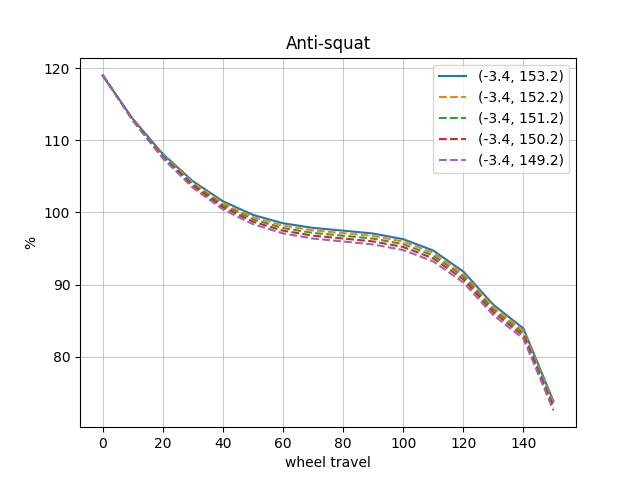
\includegraphics[scale=0.6]{anti-squat_y-.png}
        \caption{Anti-squat y座標減少}
        \label{fig_antisquat_y-:scale}
    	\end{figure}
    	
    	
    	\newpage
    	\begin{flushleft}
    	\fourteen {圖\ref{fig_antisquat_x-y+:scale}為Point4 在x座標往負x方向y座標往正y方向移動時所得到Anti-squat評比結果,由該圖可知當Point4在x座標往負方向及y座標往正y方向移動時所得到的結果會越偏離100\%。}
    	\end{flushleft}
      \begin{figure}[hbt!]
        \centering
        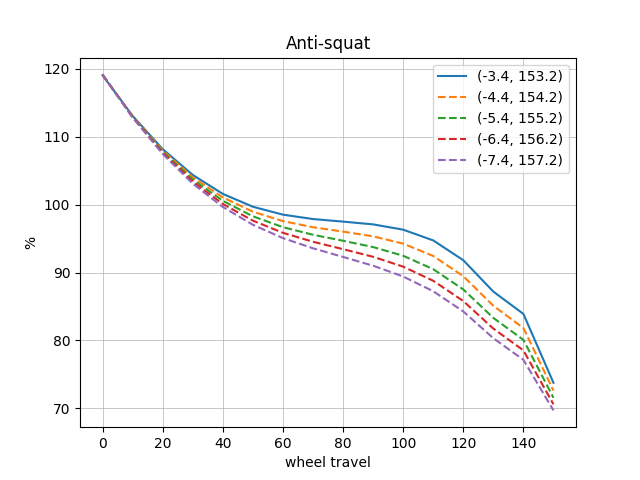
\includegraphics[scale=0.6]{anti-squat_x-y+.png}
        \caption{Anti-squat x座標減少 y座標增加}
        \label{fig_antisquat_x-y+:scale}
    	\end{figure}
    	   	
    	
    	\begin{flushleft}
    	\fourteen {圖\ref{fig_antirise_x-:scale}為Point4 在x座標往負x方向移動時所得到Anti-rise評比結果,由該圖可知當Point4在x座標往負方向移動時所得到的結果會越來越比原來的位置差。}
    	\end{flushleft}
      \begin{figure}[hbt!]
        \centering
        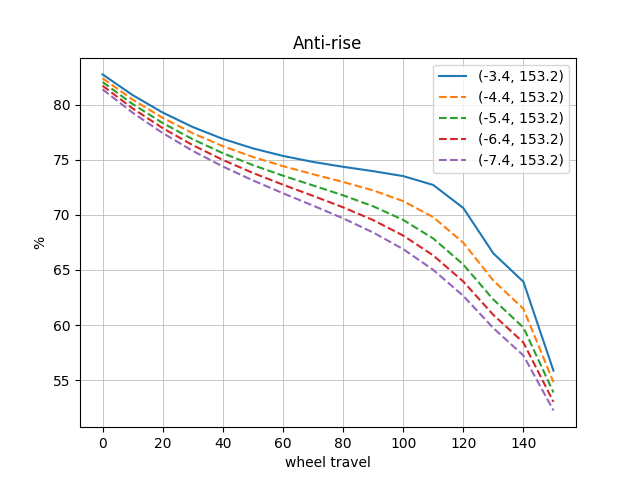
\includegraphics[scale=0.6]{anti-rise_x-.png}
        \caption{Anti-rise x座標減少}
        \label{fig_antirise_x-:scale}
    	\end{figure}
    	
    	 \newpage
    	 \begin{flushleft}
    	 \fourteen {圖\ref{fig_antirise_y-:scale}為Point4 在y座標往負y方向移動時所得到Anti-rise評比結果,由該圖可知當Point4在y座標往負方向移動時所得到的結果會越來越比原來的位置差。}
    	 \end{flushleft}
      \begin{figure}[hbt!]
        \centering
        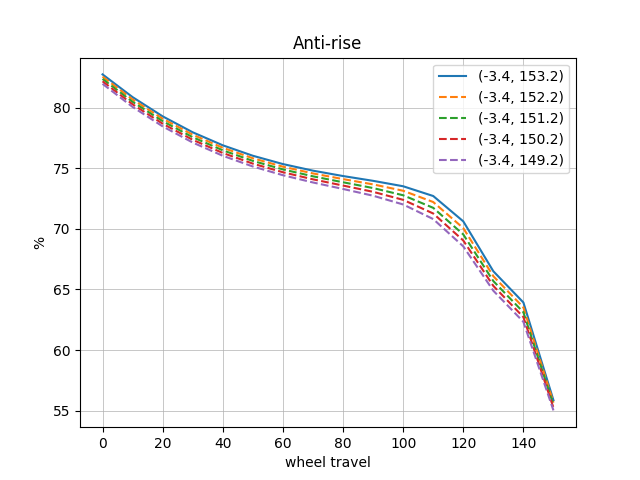
\includegraphics[scale=0.6]{anti-rise_y-.png}
        \caption{Anti-rise y座標減少}
        \label{fig_antirise_y-:scale}
    	\end{figure}
    	
    	
    	\begin{flushleft}
    	\fourteen {圖\ref{fig_antirise_x-y+:scale}為Point4 在x座標往負x方向及y座標往正y方向移動時所得到Anti-rise評比結果,由該圖可知當Point4在x座標往負x方向及y座標往正方向移動時所得到的結果會越來越比原來的位置差。}
    	\end{flushleft}
      \begin{figure}[hbt!]
        \centering
        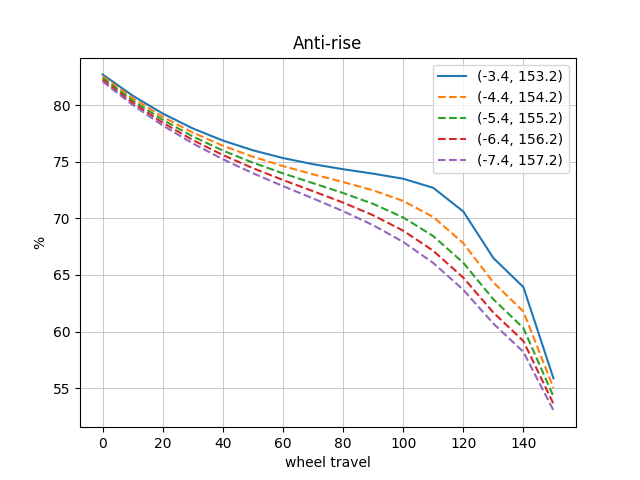
\includegraphics[scale=0.6]{anti-rise_x-y+.png}
        \caption{Anti-rise x座標減少 y座標增加}
        \label{fig_antirise_x-y+:scale}
    	\end{figure}
    	
    	\subsection{3D零件自動生成}
	\begin{flushleft}
	\fourteen {完成機構設計後接著就要進入CAD階段,不過在此階段常面臨突然遇到有其他的因素導致需要修改尺寸,此時若以手動將一個個零件一一重新修改會浪費許多時間,因此本專題建立一程式流程來進行參數化修改。}
	\end{flushleft}
	\begin{figure}[hbt!]
        \centering
        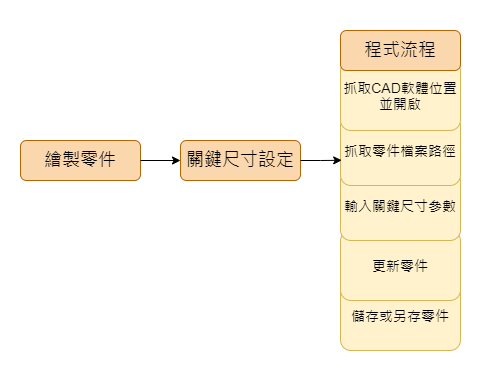
\includegraphics[scale=0.6]{3D零件生成.png}
        \caption{3D零件生成流程圖}
        \label{fig_3Dparts:scale}
    	\end{figure} 
	
	
	\begin{enumerate}
	\item{\fourteen{繪製零件:建立後續會用到的零件}
	\begin{figure}[hbt!]
        \centering
        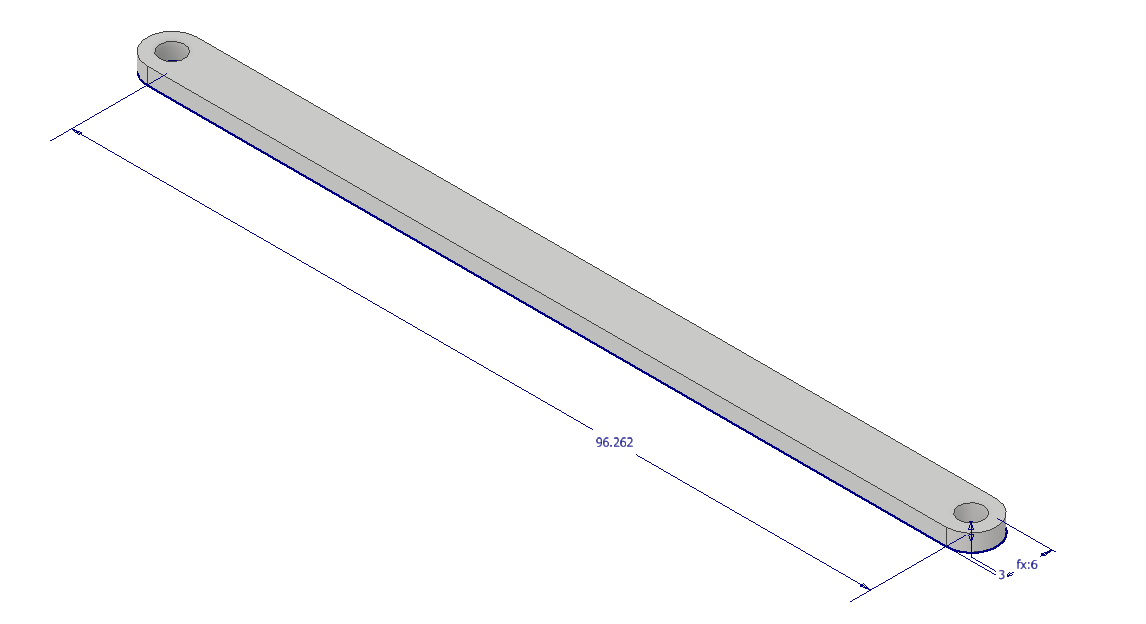
\includegraphics[scale=0.4]{binary_link.png}
        \caption{二接頭連桿}
        \label{fig_binary_link:scale}
        
        \centering
        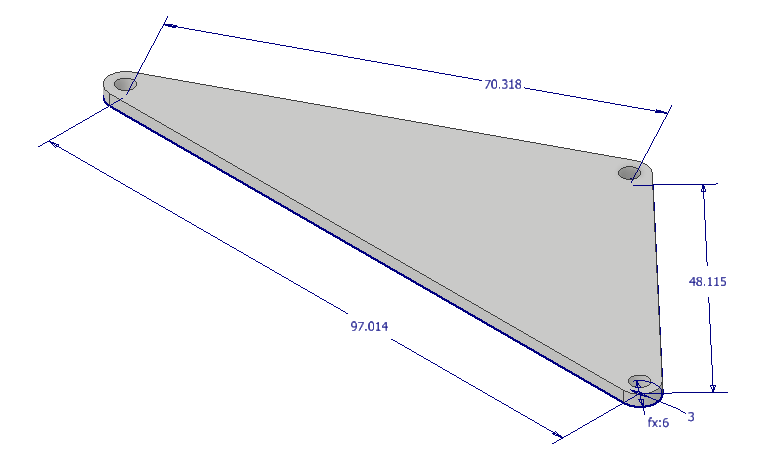
\includegraphics[scale=0.5]{ternary_link.png}
        \caption{三接頭連桿}
        \label{fig_ternary_link:scale}
    \end{figure}
    }
    
	
	\item
	{
	\begin{flushleft}
	\fourteen{關鍵尺寸設定:將所需要的零件關鍵尺寸找出並在CAD軟體中建立該參數}
	\end{flushleft}
	}
	
	\item{
	\begin{flushleft}
	\fourteen{程式流程:該流程主要以pywin32模組來完成,其中會利用該模組找到在電腦中的CAD軟體並開啟接著將找到要修改的零件模型的路徑並開啟,再將前面設定完成的尺寸參數名稱帶入函式中並輸入想要的數值,修改完畢後再更新零件才能在CAD軟體中看到修改後的變化,最後進行儲存的動作}    	
    \end{flushleft}
    }
    	
    % %%%% test the subfigure syntax
	%\begin{figure}
	%\centering
	%$\subfigure$[binary_link]{\label{fig:a} 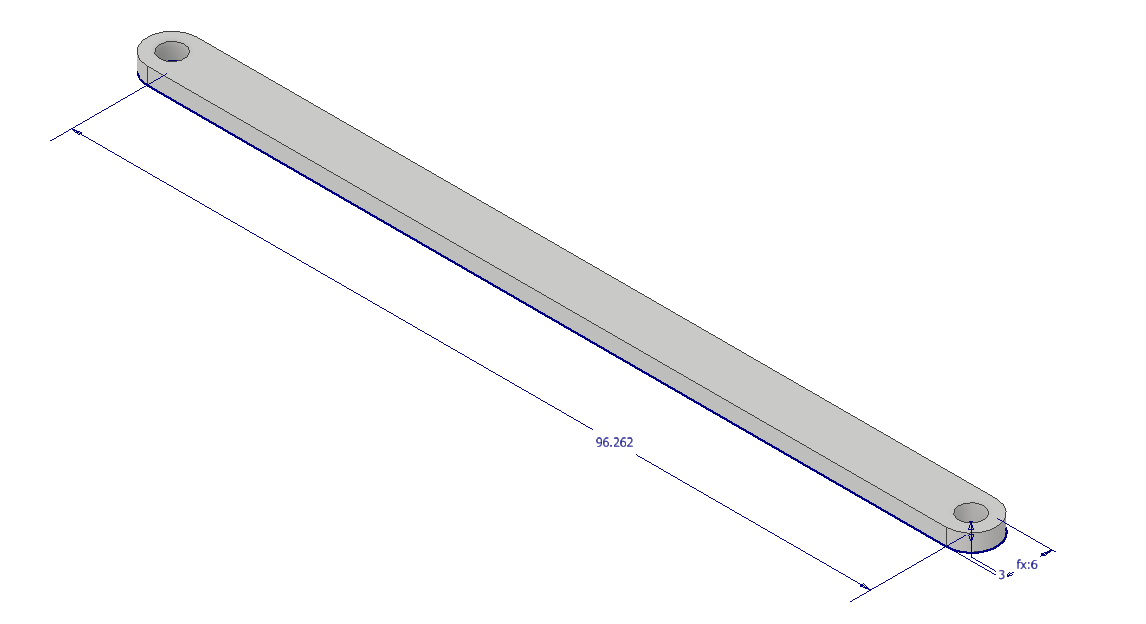
\includegraphics[width=60mm]{binary_link.png}}$
	%$\subfigure$[ternary_link]{\label{fig:b} 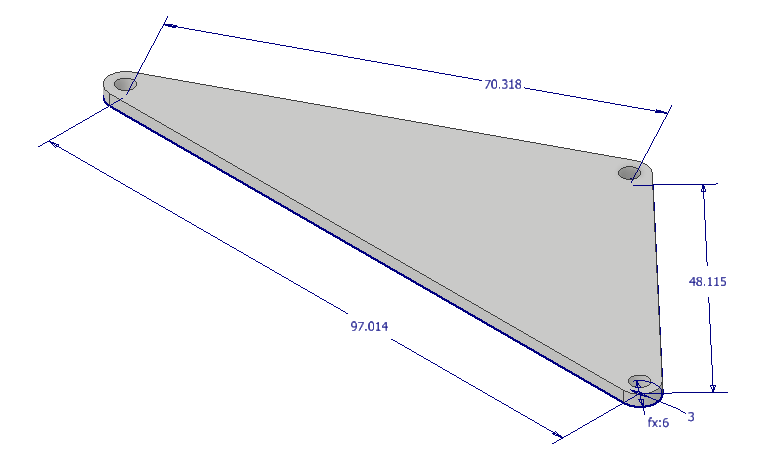
\includegraphics[width=60mm]{ternary_link.png}}$
	%\caption{my caption}
	%\end{figure}
	\end{enumerate}
    	
    	
        \chapter{結論}
        {\begin{flushleft}
        \quad \quad \fourteen {對於科技的迅速進步,開源已成了當今趨勢,因此本專題所用的套件不僅能達到其他平面機構套件大部分所擁有的功能但又有公開原始碼的優勢因此在後續的發展應該會比相對封閉的套件更加快速。而在CAD當中常有許多相似專案但是每次繪製不同零件時又要從頭開始繪製的情形,此時若沒有一套程式流程將會產生高耗時的問題,因此在本專題中所建立的自動3D零件生成以及後續利用xml檔完成組立、碰撞設定、馬達轉軸輸出設定......再直接匯入至動態分析套件減少了很多我們在進行不同機構範例分析的時間。後續Pyslvs-UI若能有更多的機構類型或是做後續的CAE分析應該能有更完整的設計流程。}
        \end{flushleft}

        \chapter{未來研究建議}
        {\begin{flushleft}
        \fourteen {本專題以已建立一流程從尺寸合成至動態模擬軟體進行運動模擬,後續可將運動系統改為動力系統並利用有限元素法對該避震機構進行受力情況的分析。}
        \begin{figure}[hbt!]
        \centering
        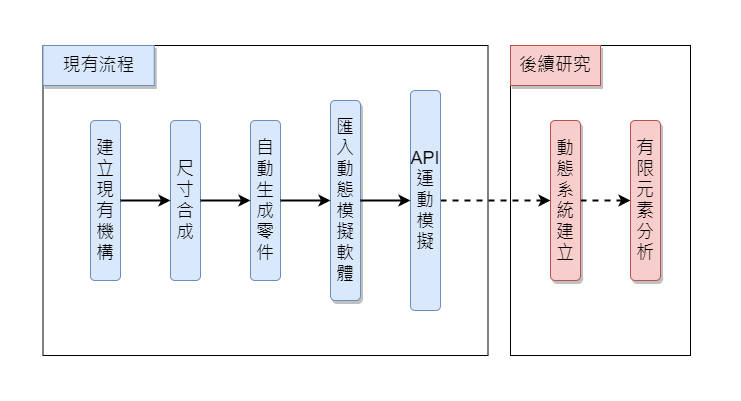
\includegraphics[scale=0.6]{follow-up research.png}
        \caption{後續研究}
        \label{fig:scale}
    	\end{figure}
        \end{flushleft}
        
        \newpage
        \addcontentsline{toc}{chapter}{\fourteen{附錄}}
        \addcontentsline{toc}{section}{\fourteen{LaTex}}
	\begin{center}
	\twenty \bf{附錄}\\
	\end{center}
	
	 \begin{itemize} 
        \item LaTex簡介:LaTex是一套由美國計算機科學家Leslie Lamport於20世紀80年代初期所開發的排版格式,相較於Word的「所見所得」編輯模式,純文字檔的模式更像在寫程式。LaTex當初建立的宗旨,就是要能完美排版文件,除了可編輯中文(簡、繁體)、英文,更可以畫圖、製表,甚至繪製五線譜和音符,基於其強大的對齊功能,LaTex已變成編輯各式文件的最佳排版方法。
		\item 特點:\\
		\end{itemize} 
		
		 \begin{enumerate}
		 \item 相容性:LaTex是免費軟體並且具有極高的可移植性,因此它幾乎可以在任何硬體平台上運行。Word有分為舊版的.doc和新版的.docx,在平台支援上,也分為for Windows和for Mac。一份在Windows上完成的文件,拿到Mac開啟,原本設定好的表格和對齊的文字都會產生變動。相較LaTex,不管是將寫好的編碼在Mac或是Windows開啟並進行編譯,最後將能得到完全相同的文件內容。
		 \item 文件排版:在處理多頁數文件時,若想將兩個不同小節互換,不僅中間每一小節在跨頁時設定好的分段都會受到影響,在進行整個區域的移動時,排版也會跑掉、長距離的圖片搬移也容易出現錯誤。且會因為快取內容即時預覽,導致向下滑動時會發生卡頓、程式短時間無法回應、甚至崩潰等情況,這些都是「前台編輯」容易發生的情況。\\
LaTex屬於「後台編輯」,因此在還沒編譯前都不會產生PDF文件,所有圖片都是以路徑方式呈現,並透過參數來設定到時的排版位置、大小和效果,因此在全部都還是編碼的情況下,調整文字位置與圖片相較容易,編輯器也不會有需要及時預覽的問題。\\
在撰寫英文文章時,LaTex也會自動幫你將每行文字數目做最佳分配,並在斷句時自動將單字從正確的音節位置分行。
		\item 編輯數學式:數學是非常重要且強大的工具。從理論推導到各式分析等,都需要數學的幫助。因此如何以最佳方式呈現數學,就成了非常重要的問題。在Word排版時,大部分都是直接用MathType,在編輯器的面板上輸入數字、選擇希臘字母、上下標後,再將其插入Word,但不易更改字型且這些公式都不帶有書籤功能,因此在內文中無法自動引用這些方程式。\\
在LaTex內進行編輯時我們只負責公式內容,公式在整份文件中的編號將會自動執行,且字型會以統一格式呈現。
	
		\begin{figure}[H]
        \centering
        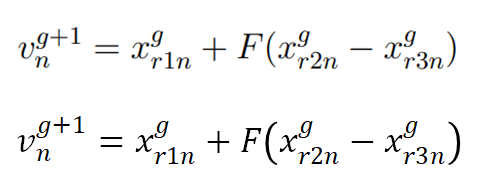
\includegraphics[scale=0.8]{公式比較圖.png} 
        \caption{公式比較圖} 
		\label{fig_公式比較圖:scale}
    	\end{figure}
    	
    	\item 巨集指令:
在LaTex內有許多巨集套件(package)可供使用,這些套件能強化環境及增加許多讓使用者進行細部微調的功能,除了引用已有套件外,也可以編寫自己的巨集(macros),為自己所需要的排版,量身訂做適合的套件。
		 \end{enumerate}
		 
		 \begin{table}[htbp] %htbp代表表格浮動位置
			\centering%表格居中
			\caption{文字編輯軟體比較表}%表:標題
			\large%字體大小
			\label{tab_文字編輯軟體比較表:scale}
			\begin{tabular}{|c|c|c|c|c|c|c|}
			\hline
			\diagbox[width=4em]& 相容性 & 直觀性 & 排版對齊 & 數學公式 & 微調細部\\ 
			\hline
			LaTeX 		&$\surd$&		&$\surd$&$\surd$&$\surd$\\
			\hline
			Word	 	&		&$\surd$&		&		&$\surd$\\
			\hline
			
			\end{tabular}
		\end{table}	
		
		 \begin{itemize}
		 \item 安裝流程:綜上所述,我們經過比較與研究最終選用LaTex編輯系統,以MikTex(系統套件)搭配Texmaker(編譯器)作為編寫專題報告的工具。
		 
        \begin{figure}[H]
        \centering
        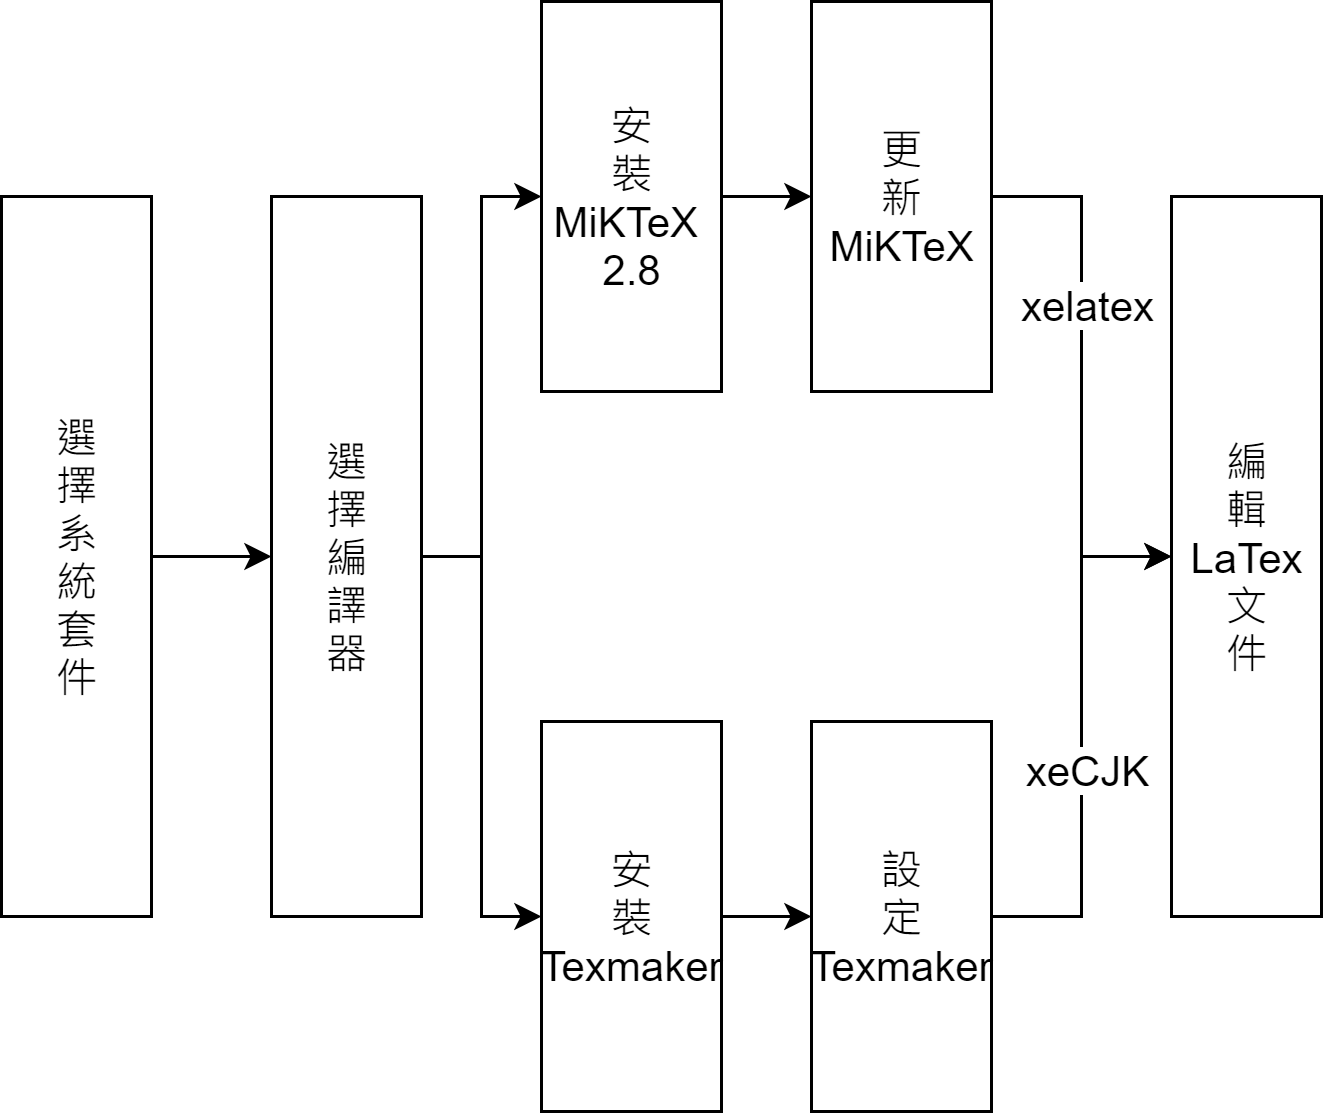
\includegraphics[scale=0.2]{LaTex安裝流程圖.png} 
        \caption{LaTex安裝流程圖} 
		\label{fig_LaTex安裝流程圖:scale}
    	\end{figure}
		 
		 \item 倉儲介紹:透過Github遠端連線協同,讓每位成員皆可在自己的電腦編譯文件,並且在倉儲內有清楚的提交紀錄與內容,在後續需要進行進度回顧或尋找某一特定版次時相較輕鬆且明確。
        
        \begin{figure}[H]
        \centering
        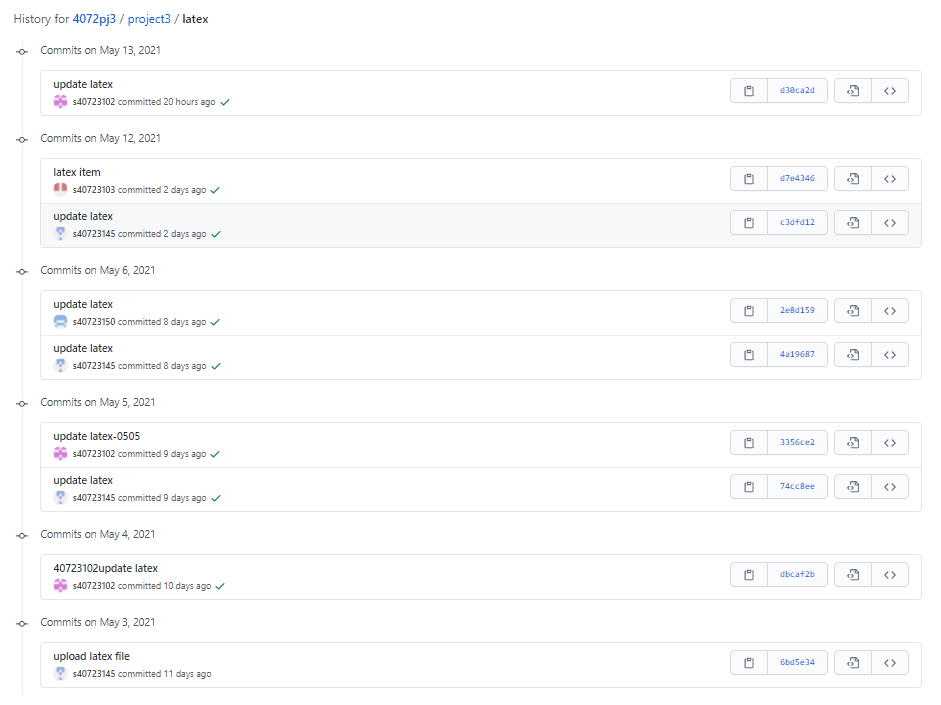
\includegraphics[scale=0.7]{倉儲推送紀錄.png} 
        \caption{倉儲推送紀錄} 
		\label{fig_倉儲推送紀錄:scale}
    	\end{figure}
    	
    	\end{itemize}
		
        \newpage
        \addcontentsline{toc}{chapter}{\fourteen{參考文獻}}
	\begin{center}
	\twenty \bf{參考文獻}\\
	\end{center}
	\begin{flushleft}
	\begin{enumerate}[1.]
	\item \quad \fourteen {"How your bike’s suspension design affects its performance on the trail" \quad https://enduro-mtb.com/en/mtb-suspension-systems/}
	\item \quad \fourteen {"What Is Anti-Squat \& How Does It Actually Affect Mountain Bike Performance" \quad https://www.pinkbike.com/news/definitions-what-is-anti-squat.html}
	\item \quad \fourteen {"Suspension Design Theory and Anti-Squat Behavior" \quad http://blog.artscyclery.com/mountain/suspension-design-theory-and-anti-squat-behavior/}
	\item \quad \fourteen {"How to Calculate Leverage Ratios" \quad https://mbaction.com/garage-files-leverage-ratio/}
	\item \quad \fourteen {"Suspension Tech: What is Anti-Rise?" \quad https://bikerumor.com/2018/10/04/suspension-tech-what-is-anti-rise/}
	\end{enumerate}
	
	
	% [2] \quad \fourteen {"What Is Anti-Squat & How Does It Actually Affect Mountain Bike Performance" \quad https://www.pinkbike.com/news/definitions-what-is-anti-squat.html}
	
    \end{flushleft}
    \newpage
    
    \addcontentsline{toc}{chapter}{\fourteen{誌謝}}
    \begin{center}
	\twenty \bf{誌謝}\\
	\end{center}

	\fourteen {德國詩人歌德曾說過:「我不應把我的作品全歸功於自己的智慧,還應歸功於我以外向我提供素材的成千成萬的事情和人物。」
	\hspace*{\fill} \\
	本研究之所以可以順利完成,首先感謝負責指導的專題教授嚴家銘老師,老師細心的指導與適時的提供建議下,確立整體研究架構與目標,更讓我們深入了解平面多連桿機構套件的理論,並在研究過程中培養我們解決問題以及獨立思考的能力。
	\hspace*{\fill} \\
	再來要感謝共同指導教授李武鉦老師,運用課堂所教導的Python程式語法,使我們在專題研究中,得以延伸學習與應用,跳脫僵化的思維去探討所要面對之問題。
	\hspace*{\fill} \\
	最後感謝學校提供完善的設備與資源,使本專題能夠圓滿完成;在專題研究上,系上提供軟硬體設備以及專題實驗室,讓我們可以利用空堂及課後時間製作與討論專題。}

    \newpage
 
    \addcontentsline{toc}{chapter}
   	{\fourteen{作者簡介}}
    \begin{center}
	\twenty \bf{作者簡介}\\
	\end{center}
	
	{\begin{textblock}{6}(0,0.5)
	\begin{figure}
	\includegraphics[width=1.15in]{st1.jpg} 
	\end{figure}
	\end{textblock}}
	{\renewcommand\baselinestretch{0.99}\selectfont %設定以下行距
	{\begin{textblock}{15}(3.5,0.7)%{寬度}(以左上角為原點之右移量,下移量)
	\noindent\fourteen \makebox[4em][s]{姓名}\enspace:\enspace
    \fourteen \makebox[4em][s]{林昱秀}\\     \hspace*{\fill} \\
    \fourteen \makebox[4em][s]{學號}\enspace:\enspace
    \fourteen \makebox[4em][s]{40723102} \\ %\makebox為文本盒子
    \hspace*{\fill} \\
    \fourteen \makebox[4em][s]{畢業學校}\enspace:\enspace
    \fourteen \makebox[9em][s]{國立虎尾科技大學}\\
    \fourteen \makebox[5em][s]{\quad}\enspace\enspace
    \fourteen \makebox[8em][s]{機械設計工程系}\\
    \hspace*{\fill} \\
    \fourteen \makebox[4em][s]{經歷}\enspace:\enspace
    \end{textblock}}}
    \hspace*{\fill} \\

	{\begin{textblock}{6}(0,2.3)
	\begin{figure}
	\includegraphics[width=1.15in]{st2.jpg} 
    \end{figure}
    \end{textblock}}
    {\renewcommand\baselinestretch{0.99}
    \selectfont %設定以下行距
    {\begin{textblock}{15}(3.5,2.5) %{寬度}(以左上角為原點之右移量,下移量)
\noindent\fourteen \makebox[4em][s]{姓名}\enspace:\enspace
\fourteen \makebox[4em][s]{林晏瑩}\\ 
\hspace*{\fill} \\
\fourteen \makebox[4em][s]{學號}\enspace:\enspace
\fourteen \makebox[4em][s]{40723103} \\ 
\hspace*{\fill} \\
\fourteen \makebox[4em][s]{畢業學校}\enspace:\enspace
\fourteen \makebox[9em][s]{國立虎尾科技大學}\\
\fourteen \makebox[5em][s]{\quad}\enspace\enspace
\fourteen \makebox[8em][s]{機械設計工程系}\\
\hspace*{\fill} \\
\fourteen \makebox[4em][s]{經歷}\enspace:\enspace
    \end{textblock}}}
    \hspace*{\fill} \\


    {\begin{textblock}{6}(0,4.1)
    \begin{figure}
        \includegraphics[width=1.15in]{st3.jpg} 
    \end{figure}
    \end{textblock}}
    {\renewcommand\baselinestretch{0.99}\selectfont %設定以下行距
    {\begin{textblock}{15}(3.5,4.3) %{寬度}(以左上角為原點之右移量,下移量)
\noindent\fourteen \makebox[4em][s]{姓名}\enspace:\enspace%\noindent指定首行不進行縮排
\fourteen \makebox[4em][s]{劉光智}\\ 
\hspace*{\fill} \\
\fourteen \makebox[4em][s]{學號}\enspace:\enspace
\fourteen \makebox[4em][s]{40723145} \\ %\makebox為文本盒子
\hspace*{\fill} \\
\fourteen \makebox[4em][s]{畢業學校}\enspace:\enspace
\fourteen \makebox[9em][s]{國立虎尾科技大學}\\
\fourteen \makebox[5em][s]{\quad}\enspace\enspace
\fourteen \makebox[8em][s]{機械設計工程系}\\
\hspace*{\fill} \\
\fourteen \makebox[4em][s]{經歷}\enspace:\enspace
    \end{textblock}}}
    \hspace*{\fill} \\

    {\begin{textblock}{6}(0,5.9)
    \begin{figure}
        \includegraphics[width=1.15in]{st4.jpg} %{}內是圖片文件的相對路徑
    \end{figure}
    \end{textblock}}
    {\renewcommand\baselinestretch{0.99}\selectfont %設定以下行距
    {\begin{textblock}{15}(3.5,6.1) %{寬度}(以左上角為原點之右移量,下移量)
\noindent\fourteen \makebox[4em][s]{姓名}\enspace:\enspace
\fourteen \makebox[4em][s]{吳佳穎}\\ \hspace*{\fill} \\
\fourteen \makebox[4em][s]{學號}\enspace:\enspace
\fourteen \makebox[4em][s]{40723153} \\ \hspace*{\fill} \\
\fourteen \makebox[4em][s]{畢業學校}\enspace:\enspace
\fourteen \makebox[9em][s]{國立虎尾科技大學}\\
\fourteen \makebox[5em][s]{\quad}\enspace\enspace
\fourteen \makebox[8em][s]{機械設計工程系}\\
\hspace*{\fill} \\
\fourteen \makebox[4em][s]{經歷}\enspace:\enspace
    \end{textblock}}}
    \hspace*{\fill} \\

    {\begin{textblock}{6}(0,7.7)
    \begin{figure}
        \includegraphics[width=1.15in]{st5.jpg} %{}內是圖片文件的相對路徑
    \end{figure}
    \end{textblock}}
    \renewcommand\baselinestretch{0.99}\selectfont %設定以下行距
    {\begin{textblock}{15}(3.5,7.9) %{寬度}(以左上角為原點之右移量,下移量)
	\noindent\fourteen \makebox[4em][s]{姓名}\enspace:\enspace
	\fourteen \makebox[4em][s]{蔡育灃}\\ \hspace*{\fill} \\
	\fourteen \makebox[4em][s]{學號}\enspace:\enspace
	\fourteen \makebox[4em][s]{40723245} \\ \hspace*{\fill} \\
	\fourteen \makebox[4em][s]{畢業學校}\enspace:\enspace
	\fourteen \makebox[9em][s]{國立虎尾科技大學}\\
	\fourteen \makebox[5em][s]{\quad}\enspace\enspace
	\fourteen \makebox[8em][s]{機械設計工程系}\\
	\hspace*{\fill} \\
	\fourteen \makebox[4em][s]{經歷}\enspace:\enspace
    \end{textblock}}
\end{document}
